\chapter{Results and Discussion}
\label{cha:3}

\section{Doping Characterization}

Upon increasing the dopant concentration deposited on top of the p(g3T2-T) film and subsequent baking, the reflection hue, as depicted in Figure \ref{fig:color} shift toward more yellowish tones.

\begin{figure}[ht]
  \centering
  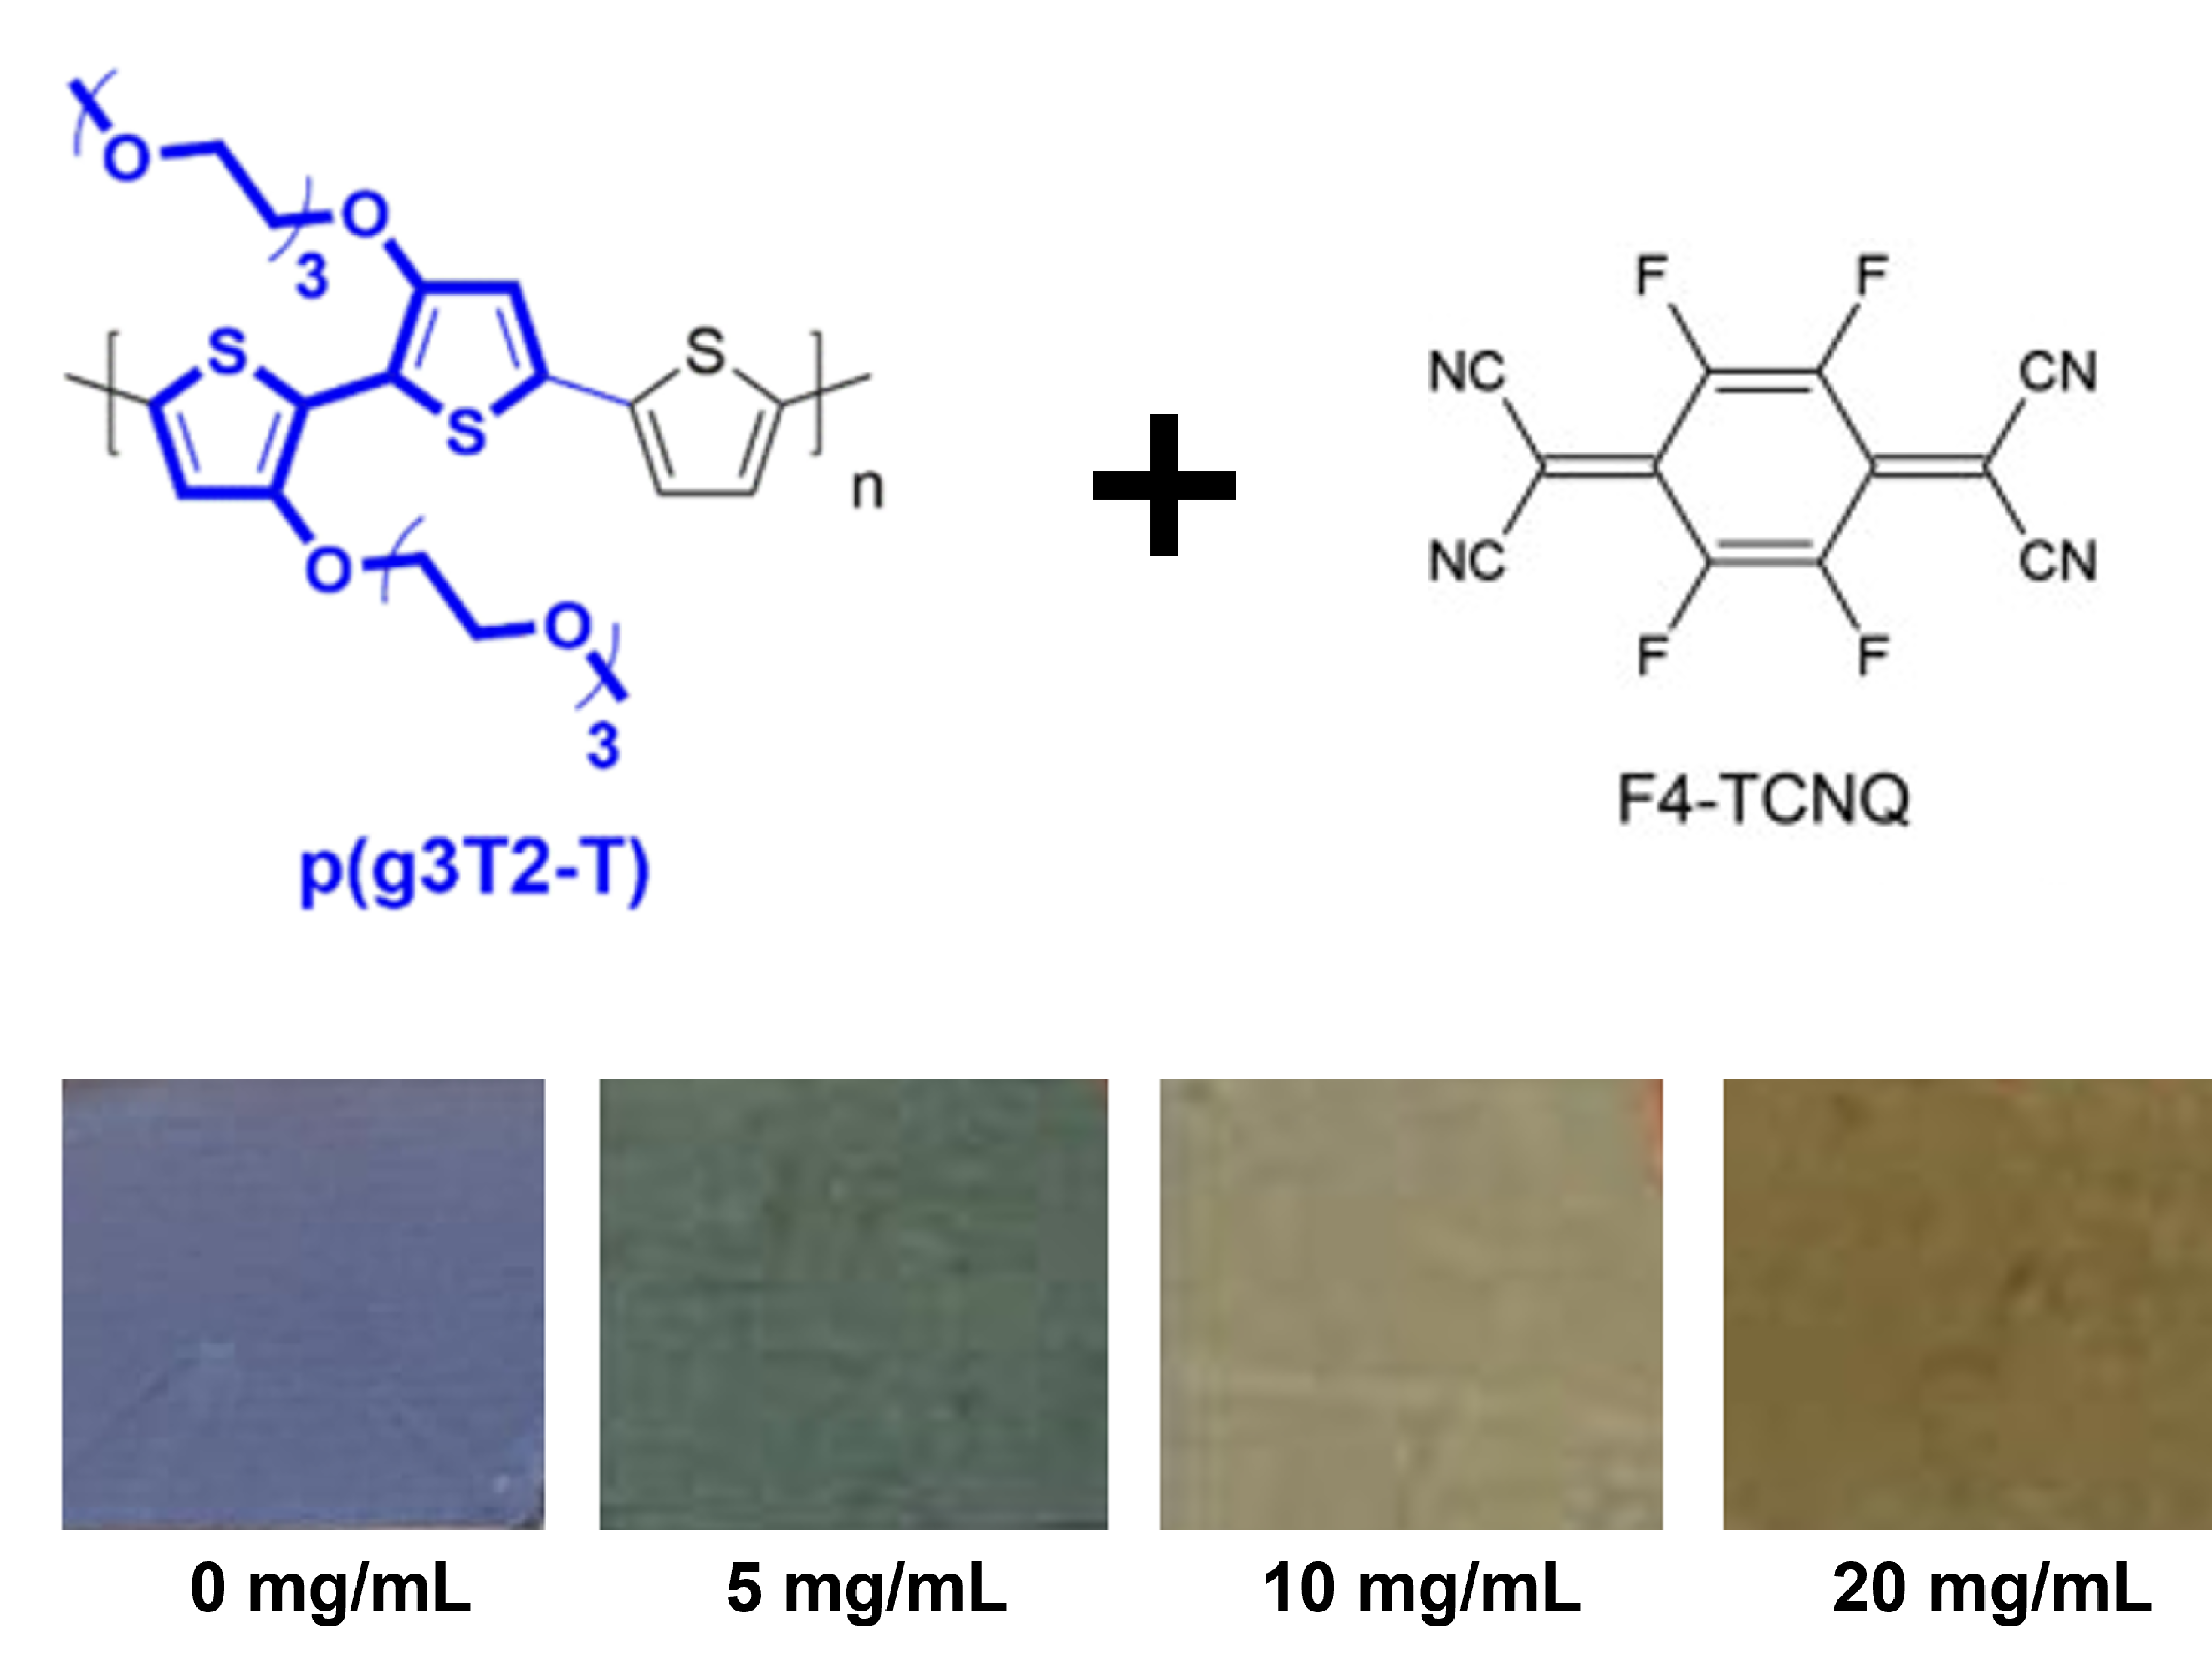
\includegraphics[width=8cm]{Images/pdf/doping_color.pdf}
  \caption[Color shift upon doping level increase]{Color change upon increasing dopant concentration from 0 to 20 mg/mL.
  \label{fig:color}}
\end{figure}

\subsection{Thickness, Sheet Resistance and Resistivity}

Sheet resistance and resistivity, as shown in Table \ref{tab:res}, were calculated using equations \ref{eq:rs} and \ref{eq:resist}, respectively, as described in previous chapter. The film thickness was determined through profilometer measurements, resulting in an approximate thickness of 70 nm.

\begin{table}[ht]
\centering
\caption{Sheet resistance and resistivity values for undoped and doped films of p(g3T2-T)}
\begin{tabular}{l|c|c|c|c}
& Undoped & 5 mg/mL & 10 mg/mL & 20 mg/mL \\\hline
R$_{S}$ ($\Omega$/sq) & 6.3M & 104.6k & 70.7k & 49.4k\\
$\rho$ ($\Omega$cm) & 44.1 & 0.73 & 0.49 & 0.35\\\hline
\end{tabular}
\label{tab:res}
\end{table}

Upon doping, a substantial decrease is observed in both sheet resistance and resistivity. However, this decrease is not as pronounced when higher dopant levels are introduced, as depicted in Figure \ref{fig:rho}. Nevertheless, when comparing the reduction among doped samples, a clear linear relationship becomes apparent with increasing the dopant concentration. 

\begin{figure}[ht]
  \centering
  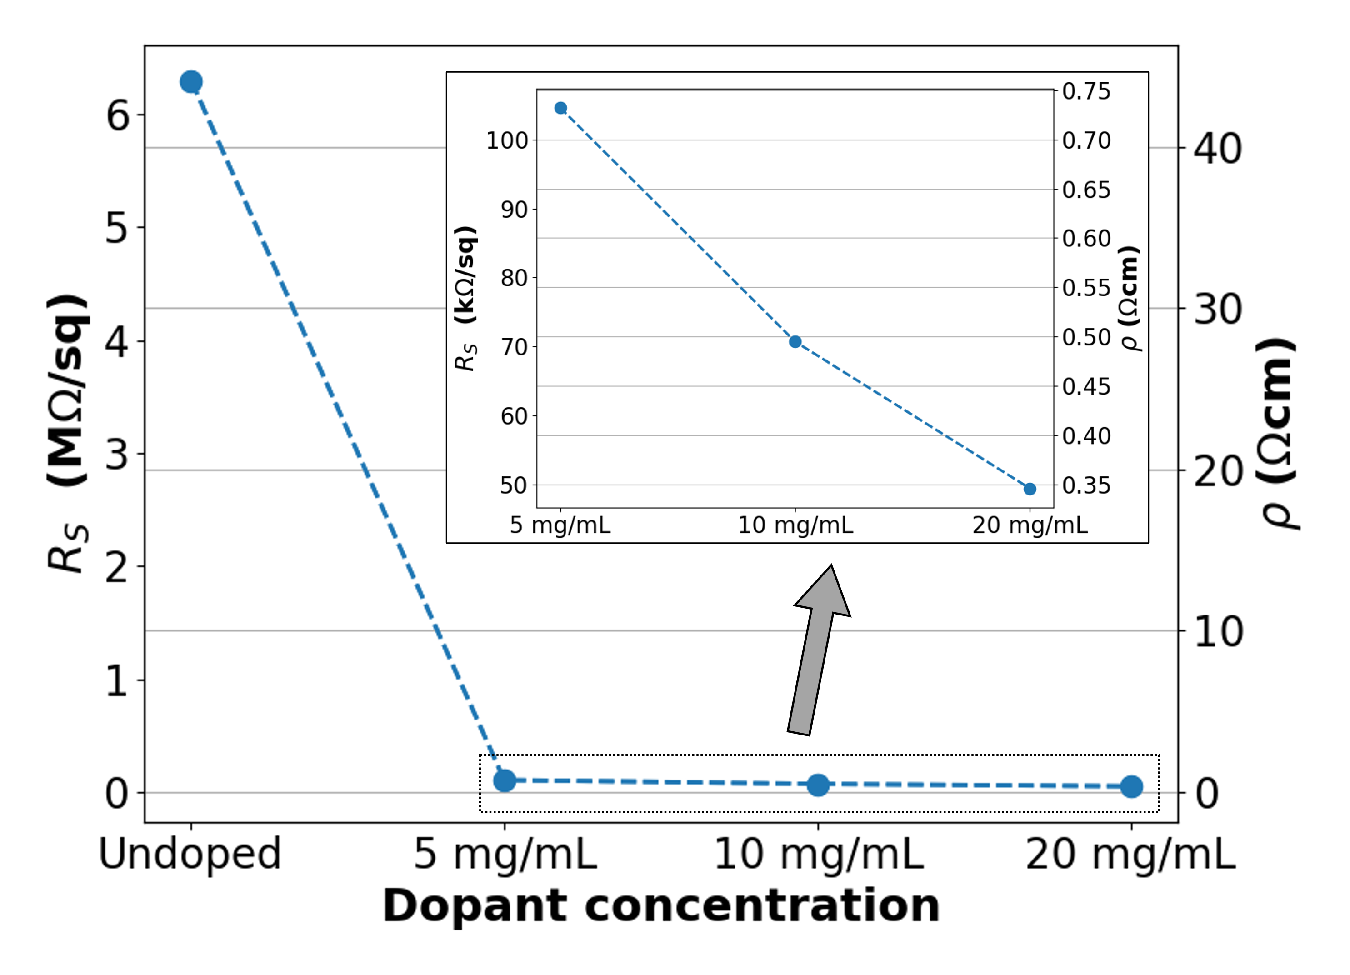
\includegraphics[width=10cm]{Images/pdf/resist+inlet.pdf}
  \caption[Sheet resistance and resistivity drop upon doping]{Sheet resistance and resistivity drop upon doping of p(g3T2-T). Inlet represents the quasi-linear drop of parameters as between doped samples.}
  \label{fig:rho}
\end{figure}


\subsection{Absorbance and Dopants Diffusion}
The visible color hue shift can be quasi-quantitatively described by examining the absorbance spectra of the samples, as illustrated in Figure \ref{fig:abs}. In the case of undoped-p(g3T2-T), there is a prominent absorption peak at 588 nm (red), which diminishes with increasing doping concentration, indicative of oxidation. Notably, new absorption peaks emerge at around 860 nm, a consequence of polaron generation, leading to new optical transitions, as explained in Chapter 2, Section \ref{subsec:moldop}. 

Tan et al. documented the appearance of new absorption peaks within the 300 to 600 nm range. The higher energy (lower wavelength) peak is generated by unreacted neutral dopant species (TCNQ$^{0}$), while the second is attributed to the new dopant anions (TCNQ$^{-}$), which induce charges in our polymer \cite{tanTuningOrganicElectrochemical2022}. Additionally, it is worth noting that, after several days of storage, the initially dominant peak of unreacted neutral dopants diminishes in intensity relative to the anions peak. This observation suggests ongoing diffusion of dopants through the polymer over time. 

\begin{figure}[ht]
  \centering
  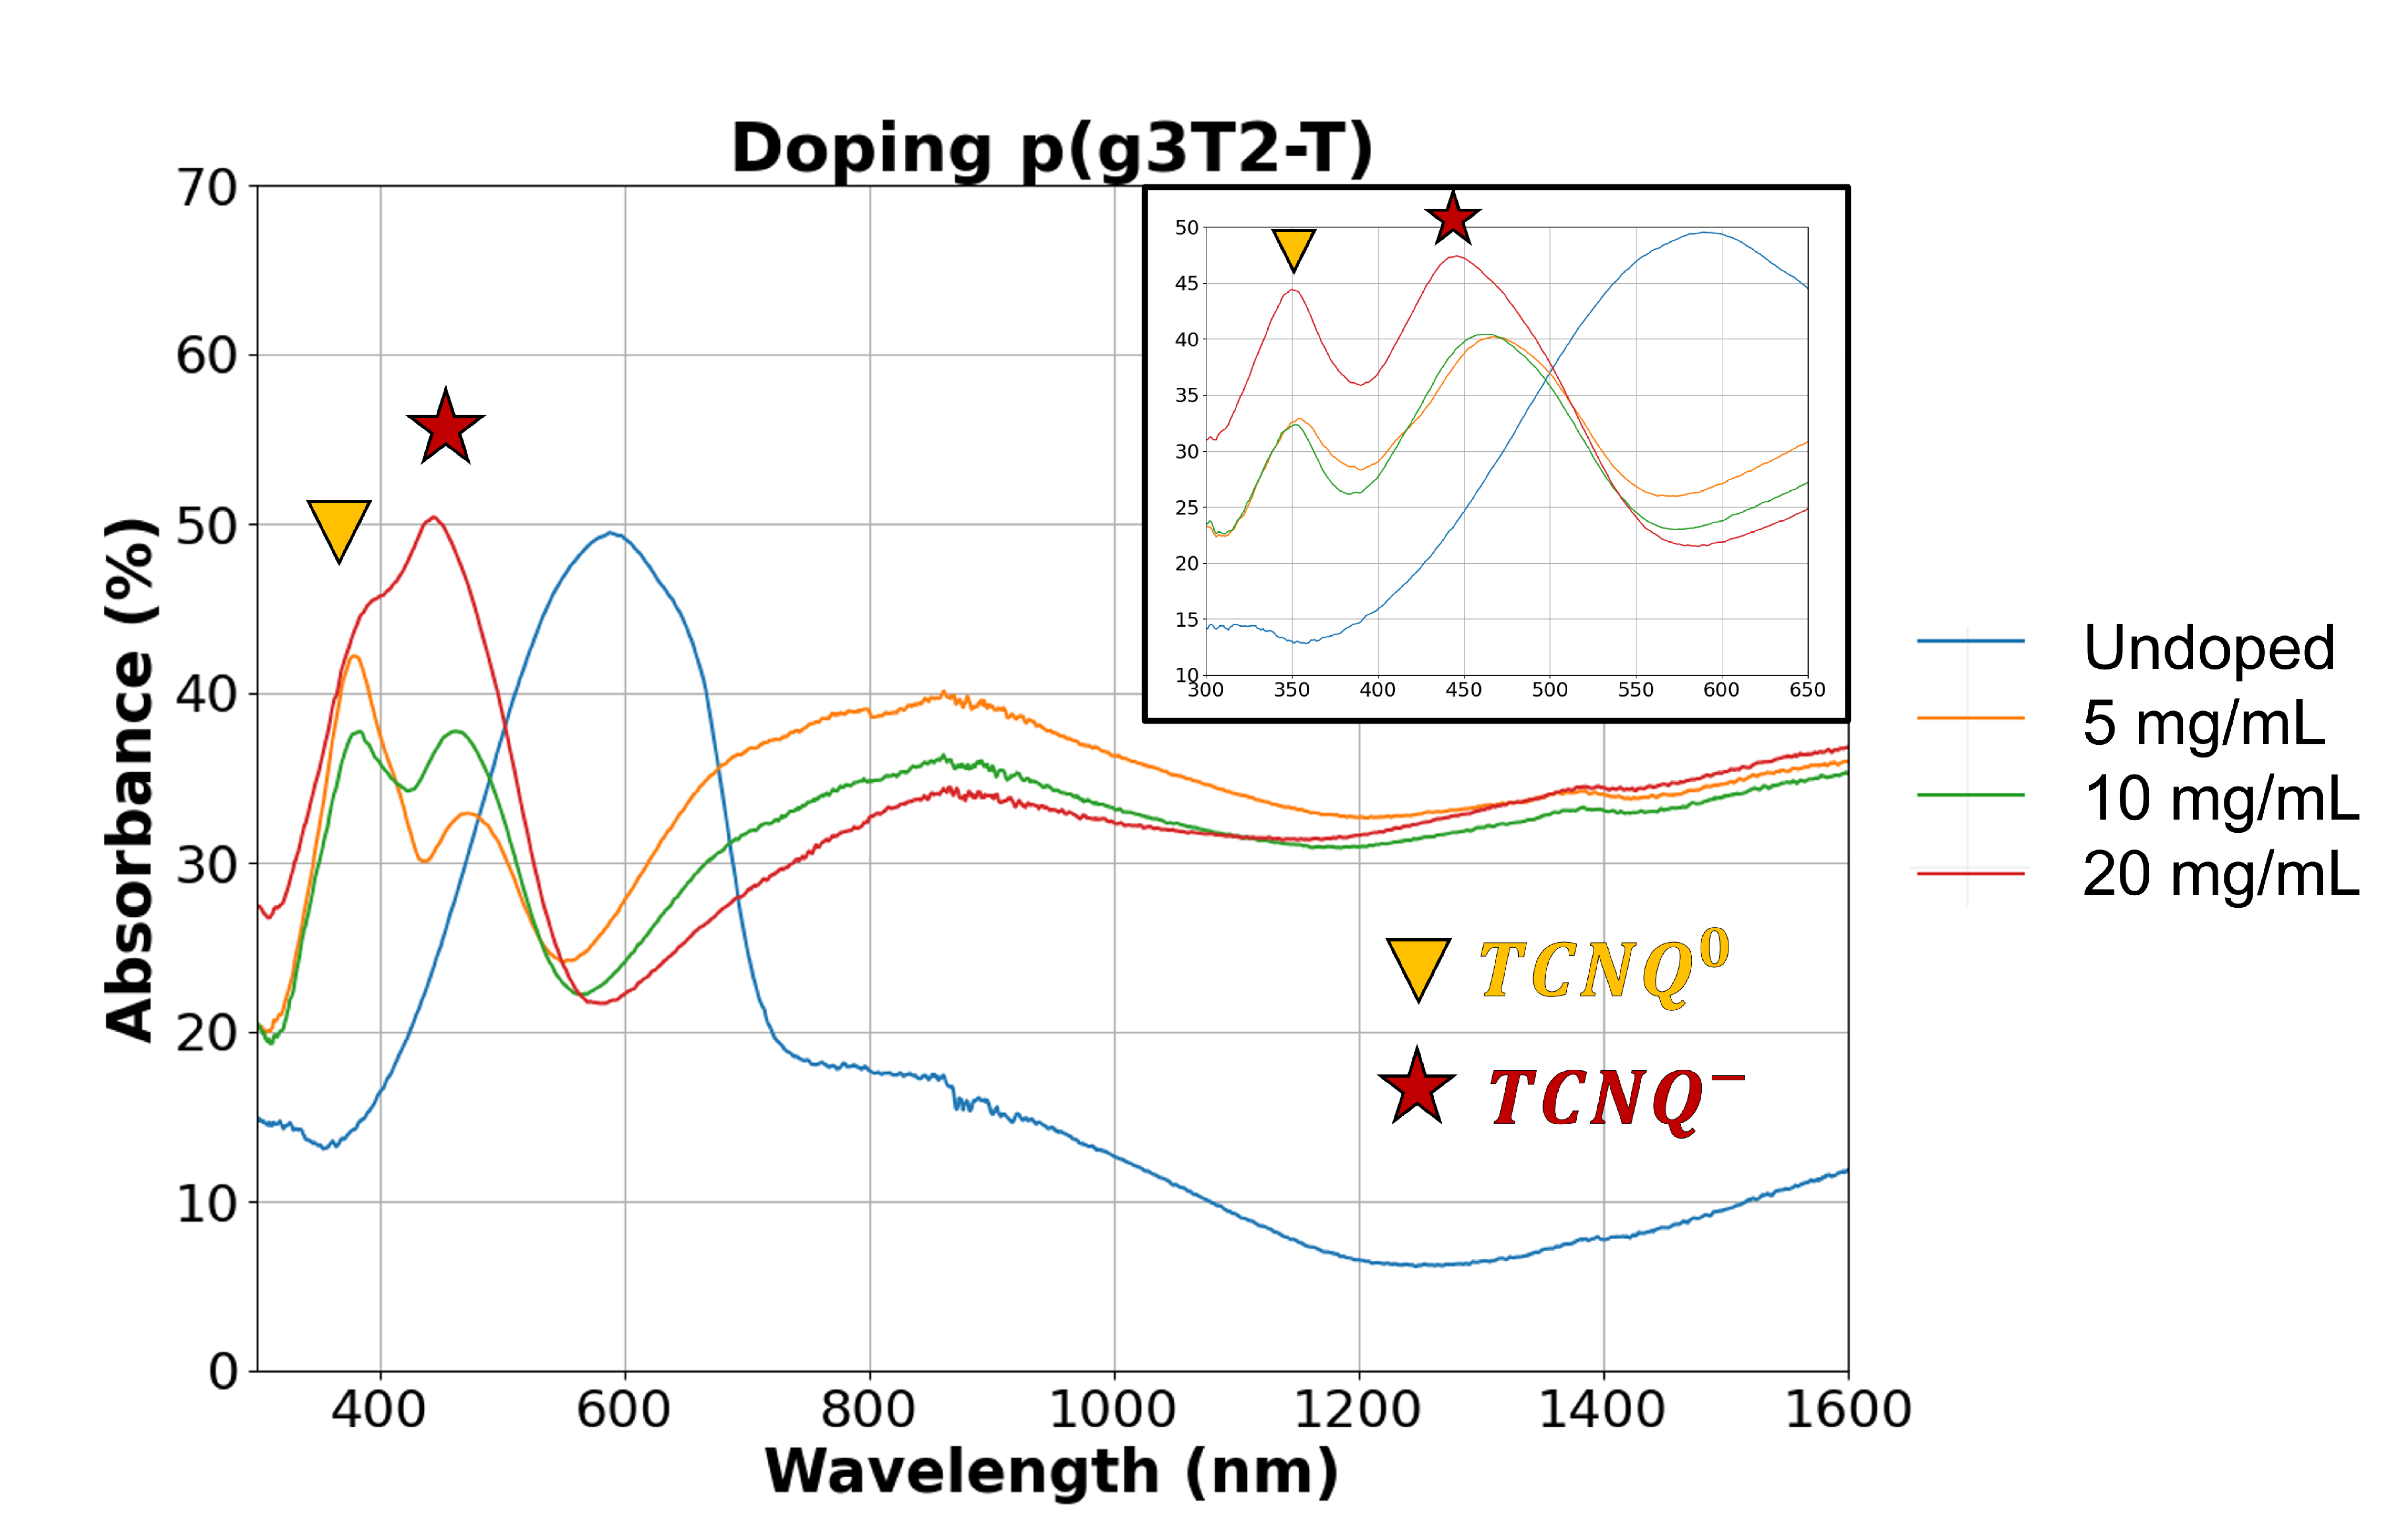
\includegraphics[width=\textwidth]{Images/pdf/abs+inlet.pdf}
  \caption[Absorbance spectra of different doping levels of p(g3T2-T)]{Spectra of undoped and doped-p(g3T2-T) at different doping levels, corresponding to samples on Figure \ref{fig:color}. Inlet represents absorbance after two weeks of storage in ambient conditions.}
  \label{fig:abs}
\end{figure}

Absorbance values are directly correlated with the density of states of these new optical transitions \cite{bredasPolaronsBipolaronsSolitons1985}. In our spectra, the absorbance value at 860 nm of the lowest-doped p(g3T2-T) sample (5 mg/mL) is relatively higher, around 40\%. This might initially appear counterintuitive. However, as the doping concentration increases, the formation of bipolarons and bipolaron bands becomes energetically more favorable \cite{enenglDopinginducedAbsorptionBands2016} . This phenomenon aligns with observations in the higher wavelengths, such as at 1600 nm, where absorbance increases in the more highly doped p(g3T2-T) sample.

Moreover, Tan et al. reported the formation of bipolaron in this specific context, evidenced by a shift to lower energies in the broad absorbance spectrum within the mid-IR region (wavenumbers 1000-1600 cm$^{-1}$) \cite{tanTuningOrganicElectrochemical2022}. Consequently, further analysis of hole bipolaron formation can be conducted with Fourier Transform InfraRed (FTIR) spectroscopy.
 
\subsection{Workfunction}

While the ideal preparation of films for studying electron energy levels with UPS involves working under inert conditions to prevent contamination, the current fabrication process of OECTs unavoidably exposes our films at ambient conditions. Therefore, measurements were conducted following deposition under these ambient conditions. Yet, it is possible to discern an increase in the workfunction, indicated by a shift of Fermi level of the polymer. This shift towards the HOMO level is more pronounced at higher dopant levels, as depicted in Figure \ref{fig:ups}, which is characteristic of p-type doping. Although some potential contamination prevented the measurement of samples with a dopant concentration of 20 mg/mL, the trend is clearly evident.

\begin{table}[ht]
\centering
\caption{Workfunction calculation from UPS measurements.}
\begin{tabular}{l|c|c|c}
& Undoped & 5 mg/mL & 10 mg/mL \\\hline
E$_{HBEC}$ [eV] & 17.35 & 16.47 & 16.36\\
E$_{HOMO}$ (vs E$_{F}$) & 4.28 & 3.27 & 3.24\\
WF [eV] & 3.87 & 4.28 & 4.86\\\hline
\end{tabular}
\label{tab:ups}
\end{table}

It is important to consider that UPS is a surface-sensitive measurement. The penetration depth of the ultraviolet-range electrons in UPS is approximately 2 nm, significantly less than our polymer thickness (approximately 70 nm). Consequently, this technique constrains our understanding of the diffusion of dopants throughout the entire volume of the polymer. While, we gained some insights into this matter in the previous subsection, further analysis could be undertaken using X-Ray Photoelectron Spectroscopy which offers a depth profiling mode. %but along with depth profiling mode 3

\begin{figure}[ht]
	\centering
	\subfloat[\textbf{}]{{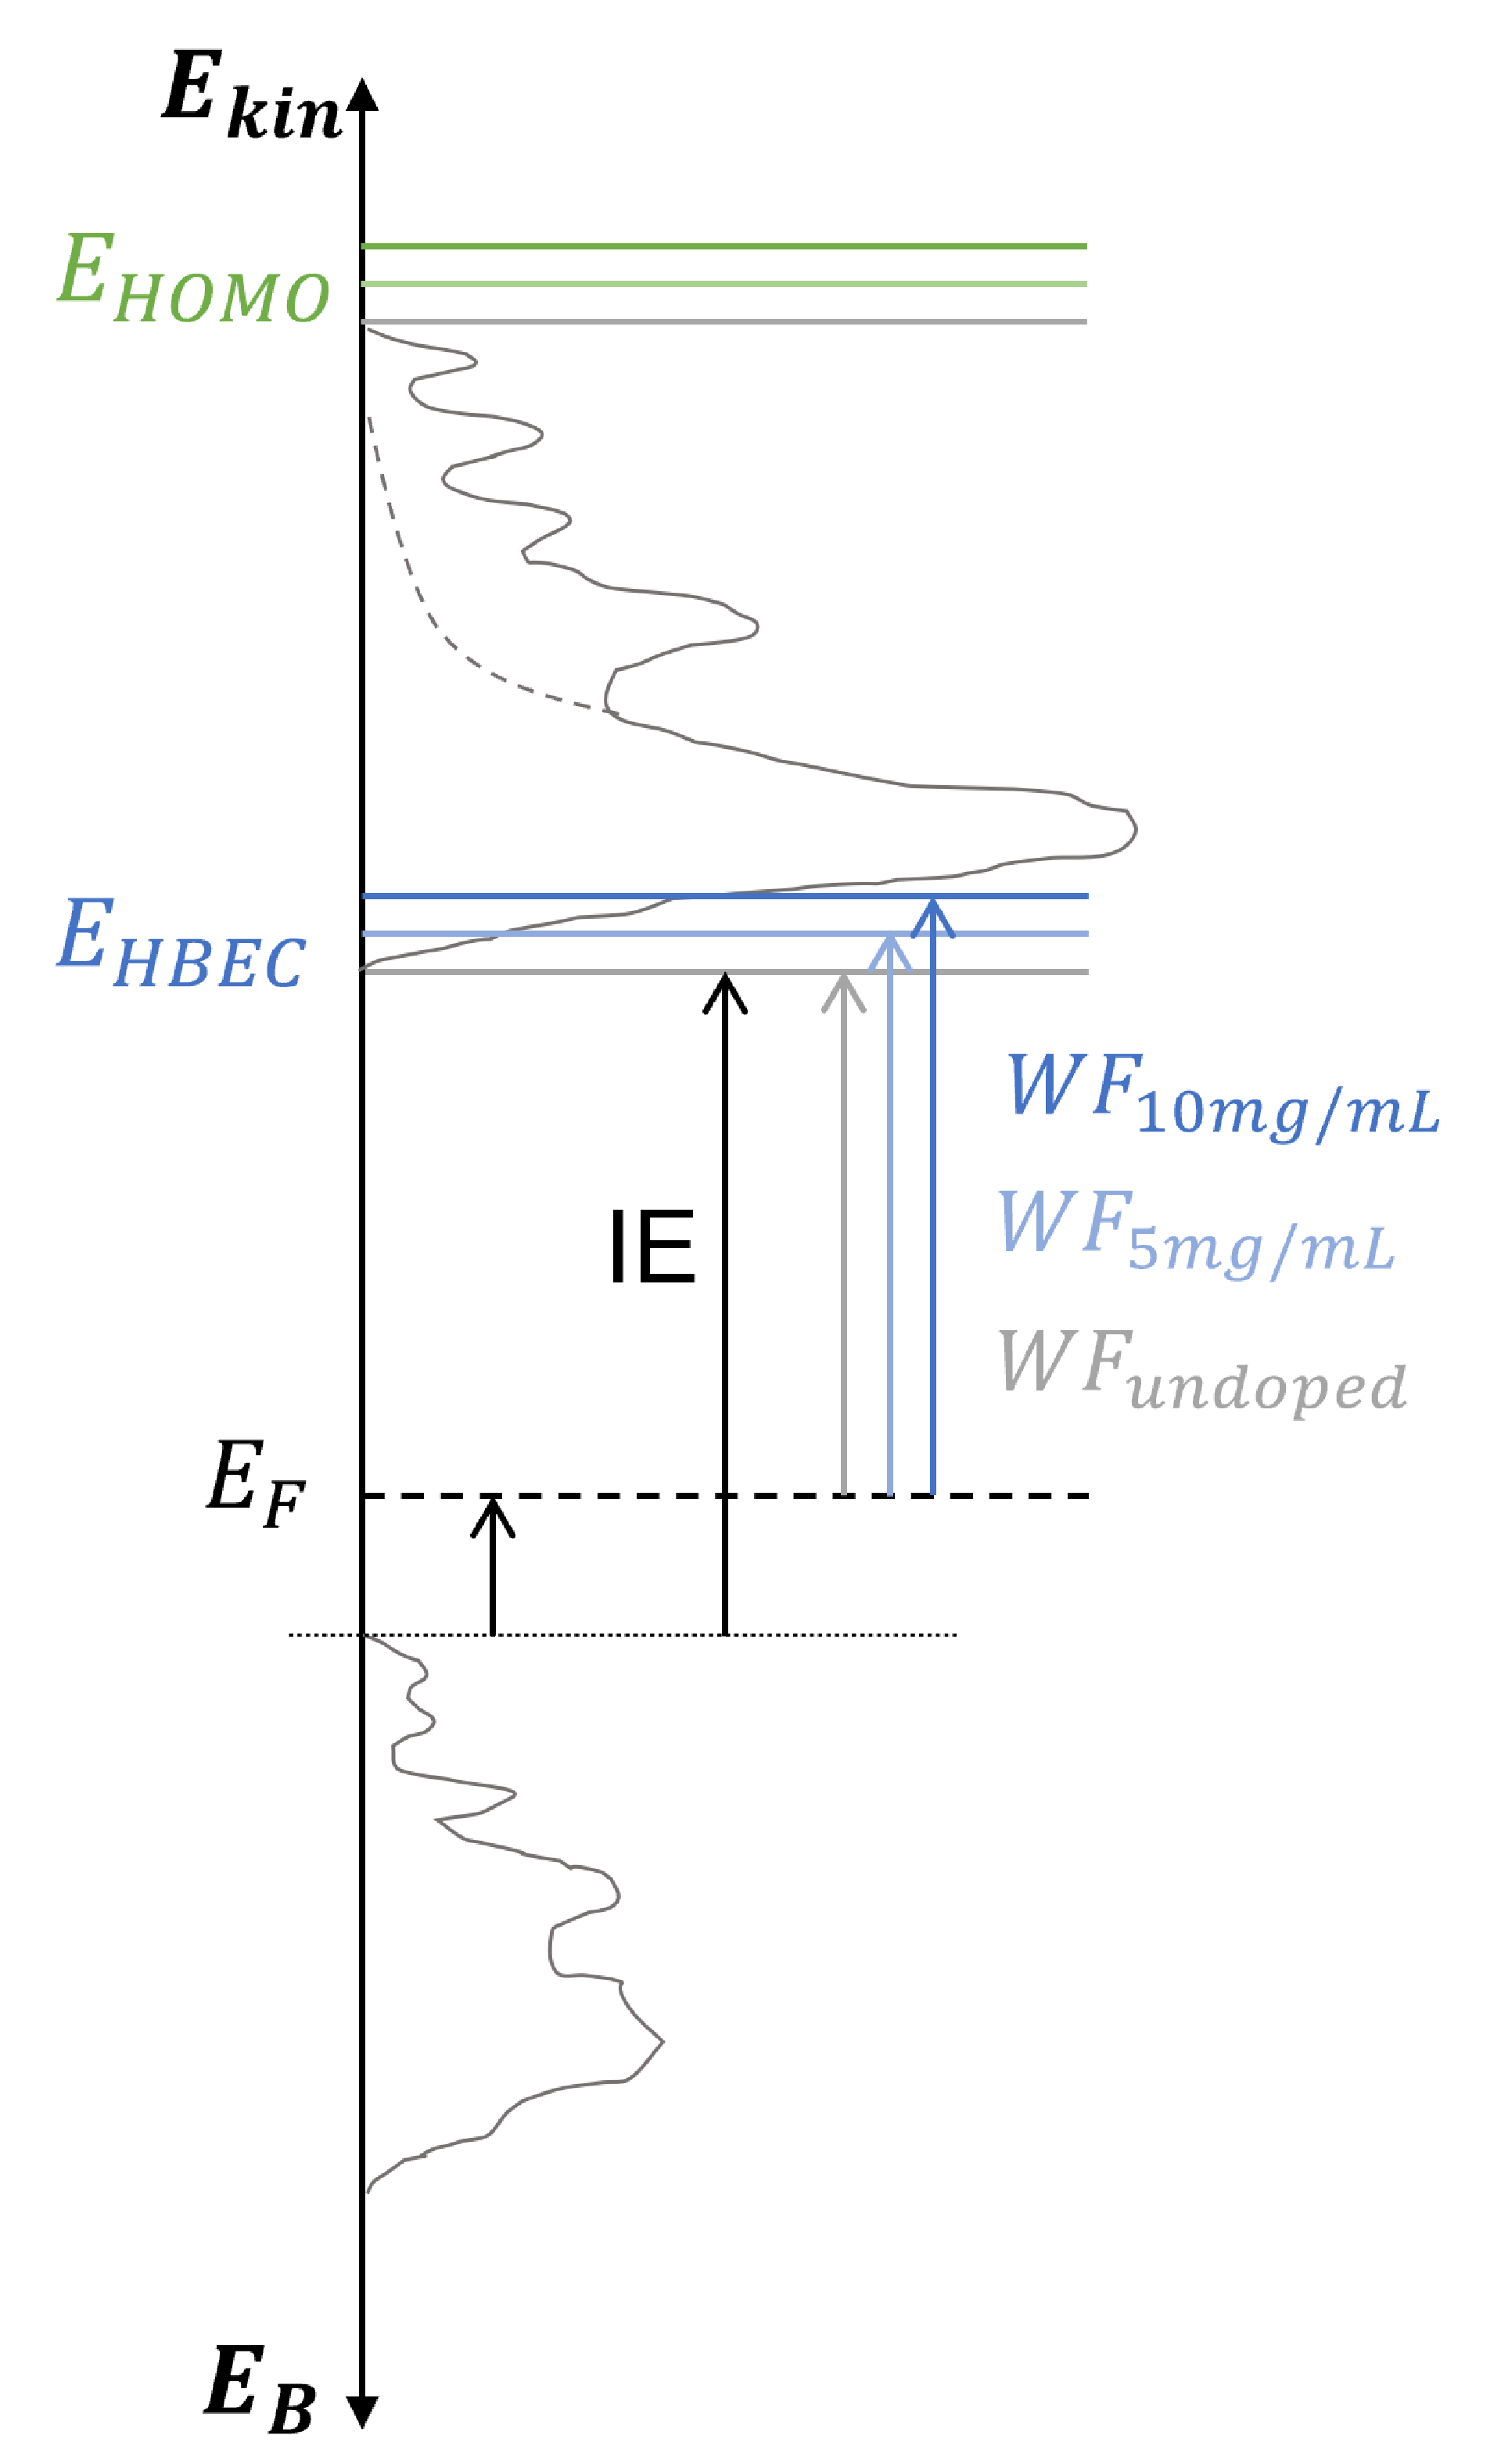
\includegraphics[width=6cm]{Images/pdf/WF_final.pdf} }}
	%\qquad
	\hspace{2em}
	\subfloat[\textbf{}]{{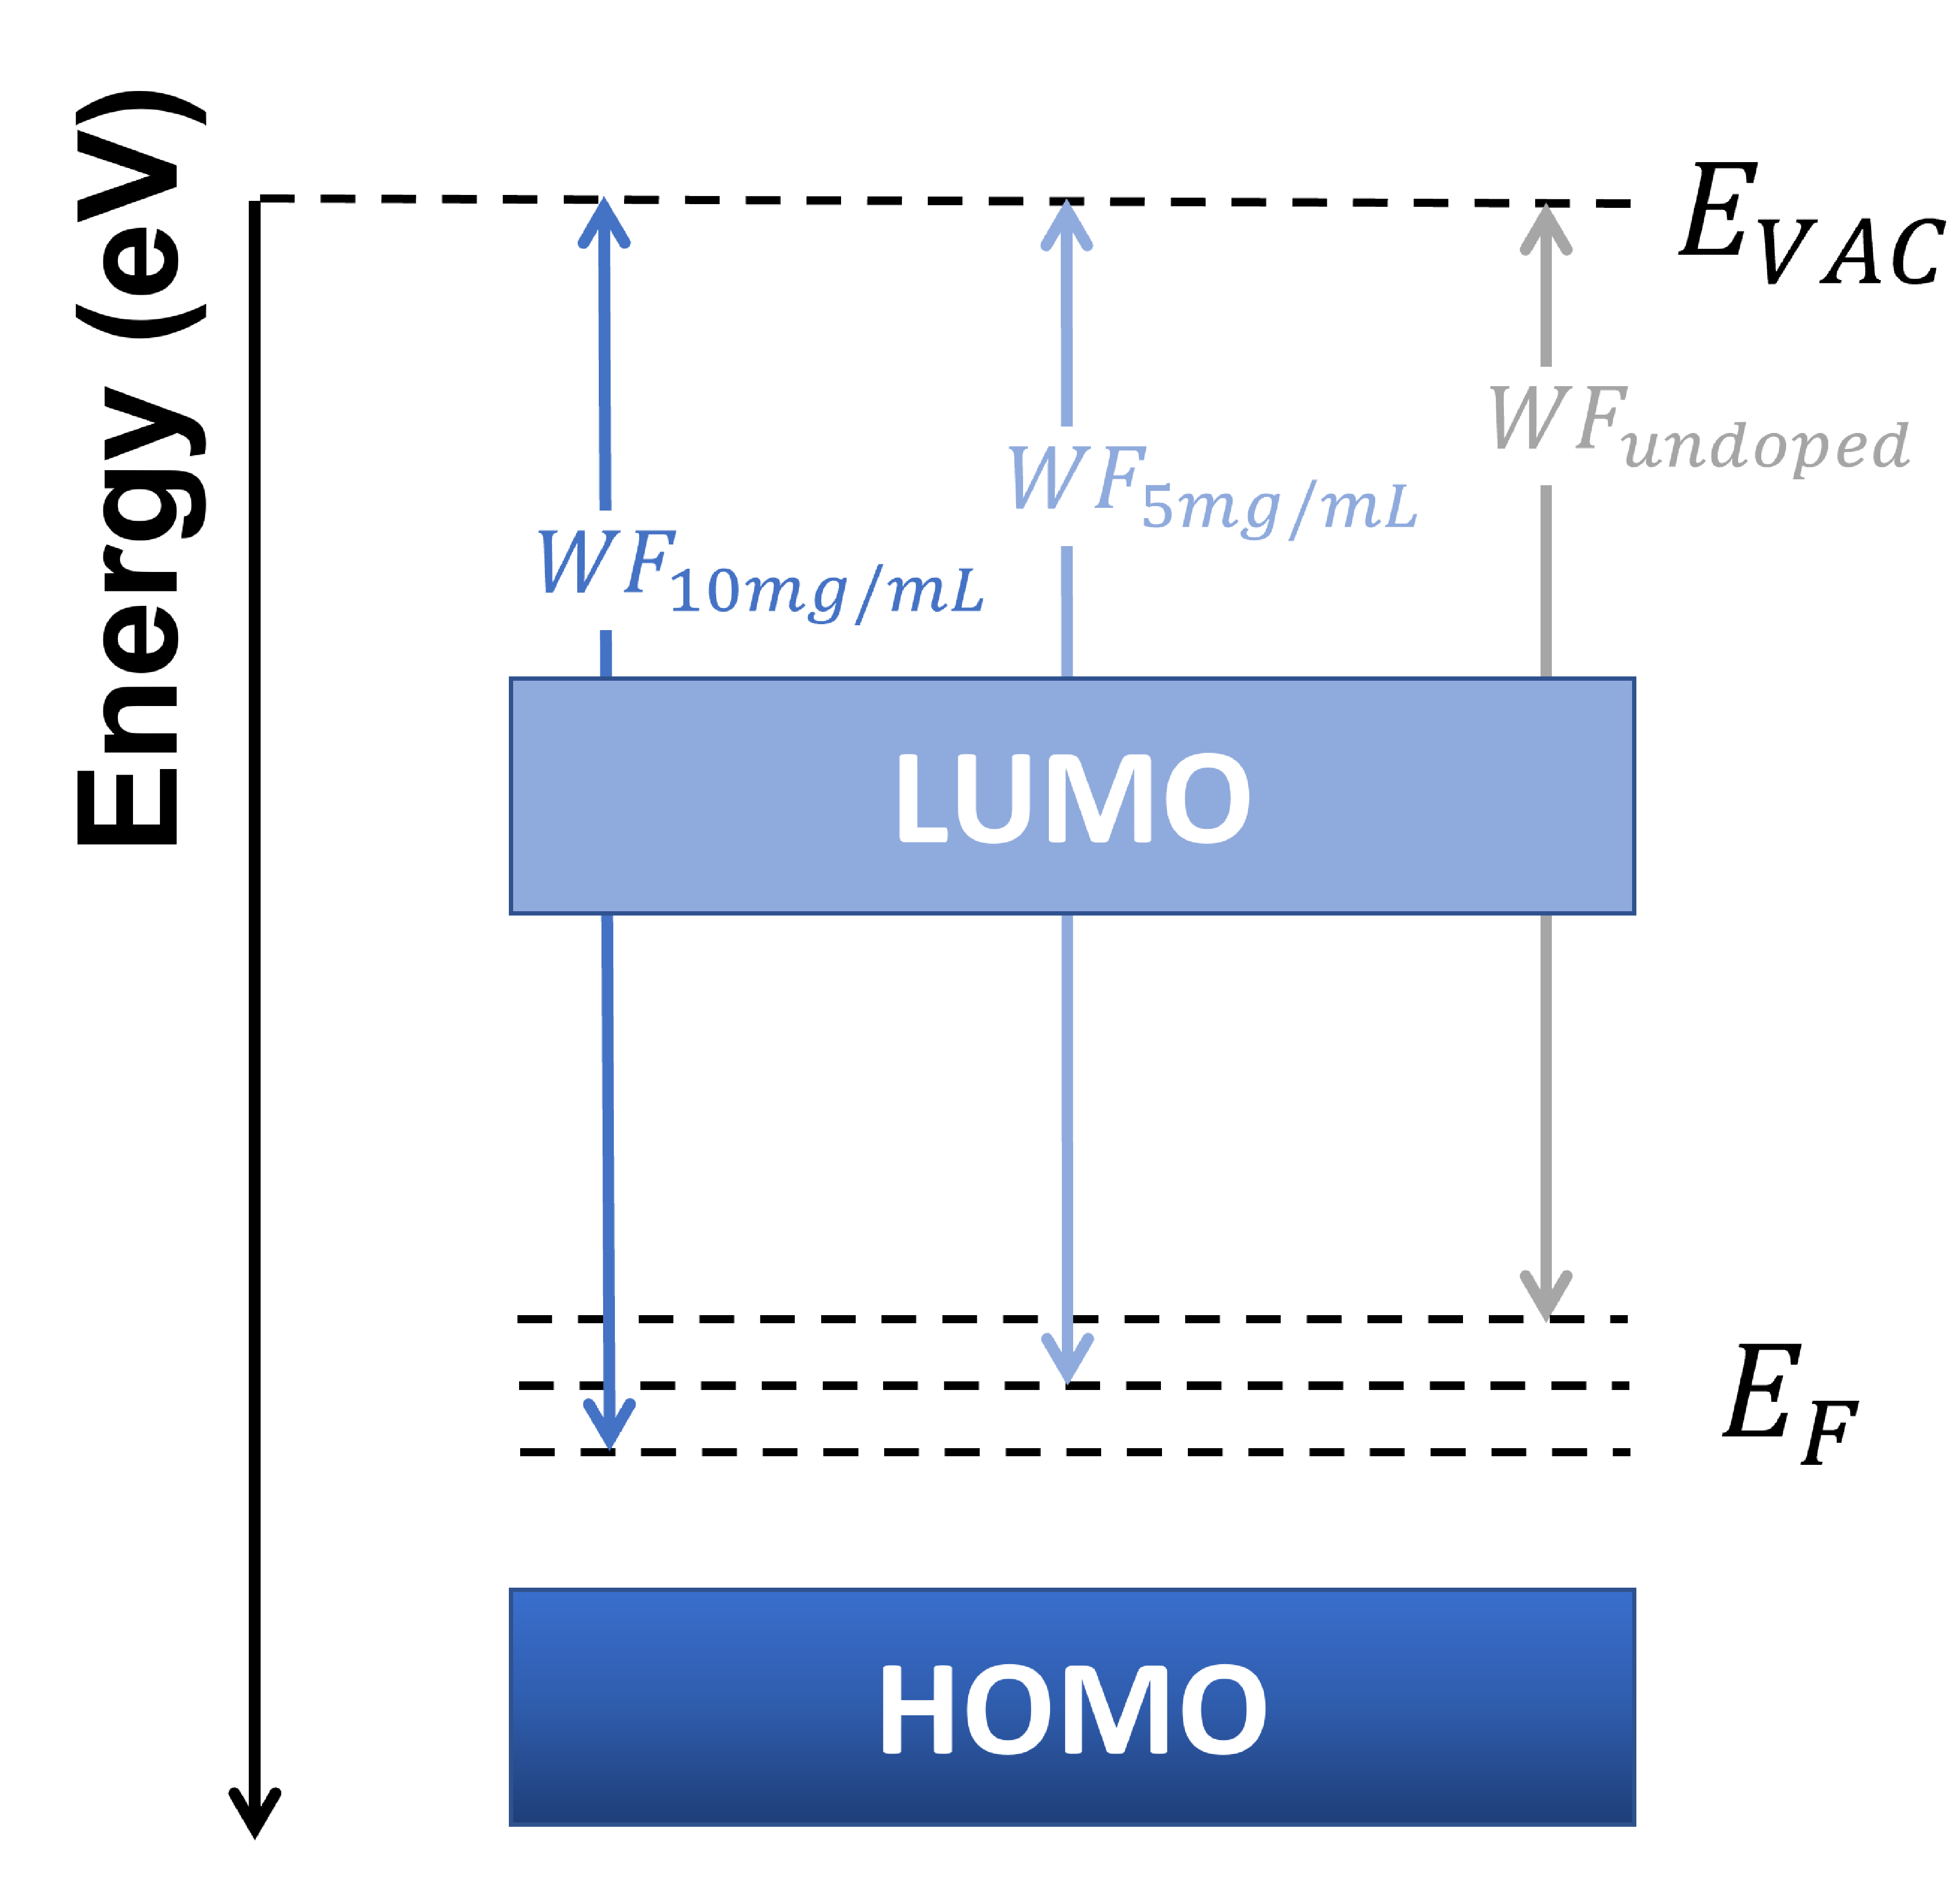
\includegraphics[width=6.5cm]{Images/pdf/WF.pdf} }}
	\caption[Representation of the Fermi level shift upon doping]{ Graphical representation of A) the relationship between the binding energies E$_{B}$ and the kinetic energy of the photoelectrons E$_{kin}$, and B) the Fermi level shift, upon doping.} 
	\label{fig:ups}
\end{figure}

%\subsection{Roughness}

\section{Fabrication of Organic Electrochemical Transistors}

%Prior biasing gate, which is due to passive (ion) diffusion?

\subsection{Influence of Doping on OECT Channel}
The fabrication process uses a mask that include a microstructure gate, suitable for studying OECTs with both channel and gate made of the same OMIEC material, commonly PEDOT:PSS. The result of the patterning process is displayed in Figure \ref{fig:channel}. 

\begin{figure}[ht]
  \centering
  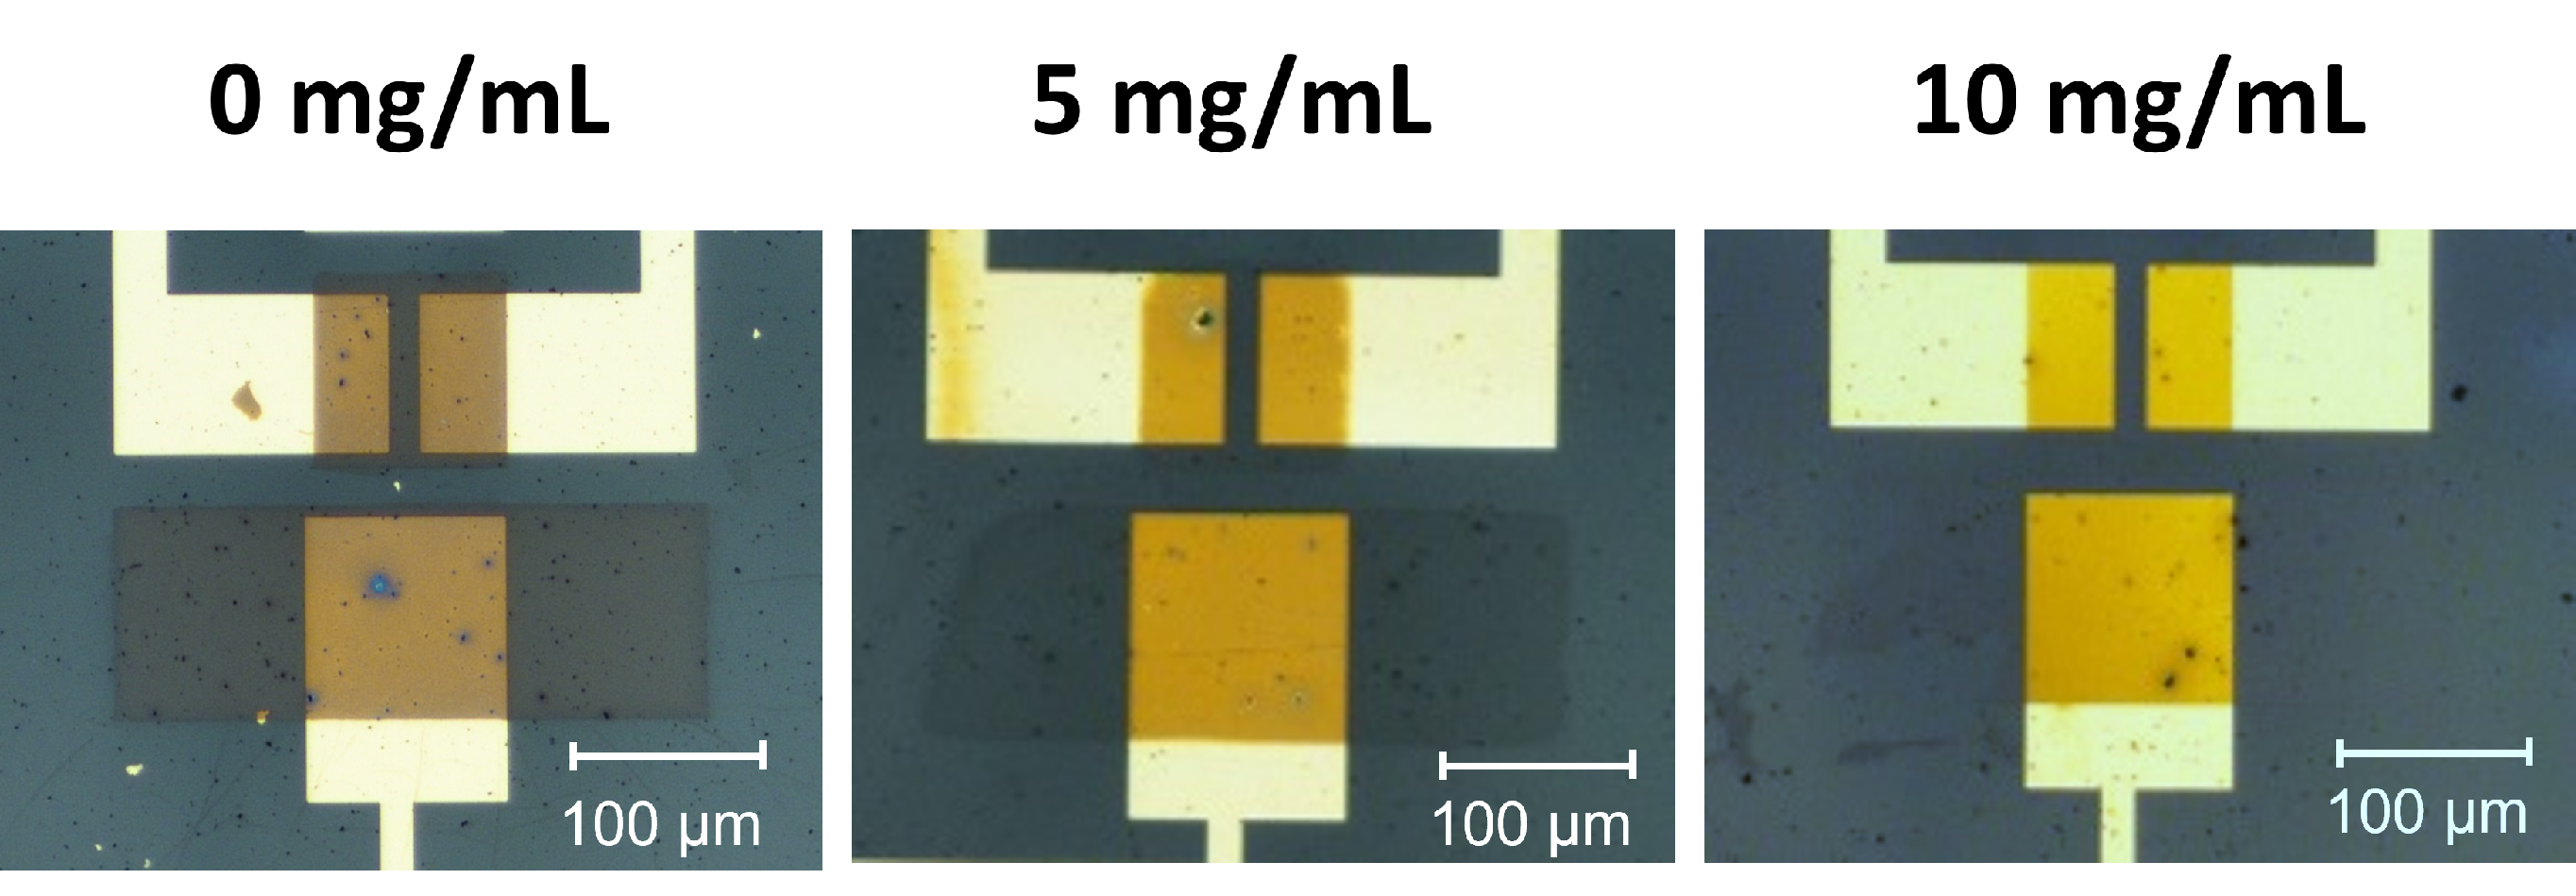
\includegraphics[width=10cm]{Images/pdf/BigGateDevices.pdf}
  \caption[Micrographs of a patterned channel and gate p(g3T2-T) at different doping levels]{Micrographs of patterned channel and gate with p(g3T2-T) undoped, 5 mg/mL and 10 mg/mL dopants, following procedures explained in Section \label{subsec:photo}.}
  \label{fig:channel}
\end{figure}

However, in this section, we will specifically examine only the OMIEC channel (p(g3T2-T)) at various doping levels paired with a non-polarizable Ag/AgCl electrode as gate, and coupled with SSE precursor.

Unfortunately, the sample that used solution with dopant concentration of 20 mg/mL exhibited doping homogeneity issues. While photolithography was still possible, it could not provide a fair basis for comparison with the other devices. Therefore, this sample will be omitted from this analysis.

The results shown in Figure \ref{fig:transx2}, Figure \ref{fig:shift1} and Figure \ref{fig:vth_vds} correspond to the same device and same loop on each sample (undoped, 5 mg/mL and 10 mg/mL dopants). Among the attempts to increase the yields, only 3 or 4 out of the 14 devices were operational on each sample. Further improvements on the development process were needed, and were accomplished as it will be shown in further sections of this chapter. After reporting the findings on these analysis, a more statistical study will be shown within the operating devices on each sample from the same batch of materials.

Transfer characteristics illustrated in Figure \ref{fig:transx2}A, C, E correspond to undoped, 5 mg/mL and 10 mg/mL dopants, respectively. A positive turn ON voltage is perceived in the undoped OECT device, which evidenced the fast oxidation (or unwanted doping) of p(g3T2-T) under environmental conditions due to its low IP. 

Gate current (I$_{GS,ON}$) is displayed in dotted lines and it is perceive that the drain OFF current (I$_{DS,OFF}$) is dominated by this leakage current in all devices. Figure \ref{fig:shift1} shows doped devices have minimum differences on I$_{DS,OFF}$, and higher values were measured in the undoped device at all V$_{DS}$ values. As it was reported by Hidalgo et al. pristine p(g3T2-T) show oxygen reduction reaction activity in oxygen-saturated conditions, increasing the current within the polymer until reaching saturation \cite{hidalgocastilloSimultaneousPerformanceStability2022a}. It will be necessary to control the oxidation state of the polymer among the different steps of the photolithography process, and somehow revert the oxidation of p(g3T2-T), this issue will be further discuss in the following sections.

The higher dopant concentration device (10 mg/mL dopant) shows signs of breakage as going to more negative V$_{DS}$ (Figure \ref{fig:transx2}E and Figure \ref{fig:shift1}D), therefore, this measurement will be disregard for transconductance and threshold voltage calculation.

\begin{figure}[!htb]
    \centering
    \subfloat[Undoped device]{{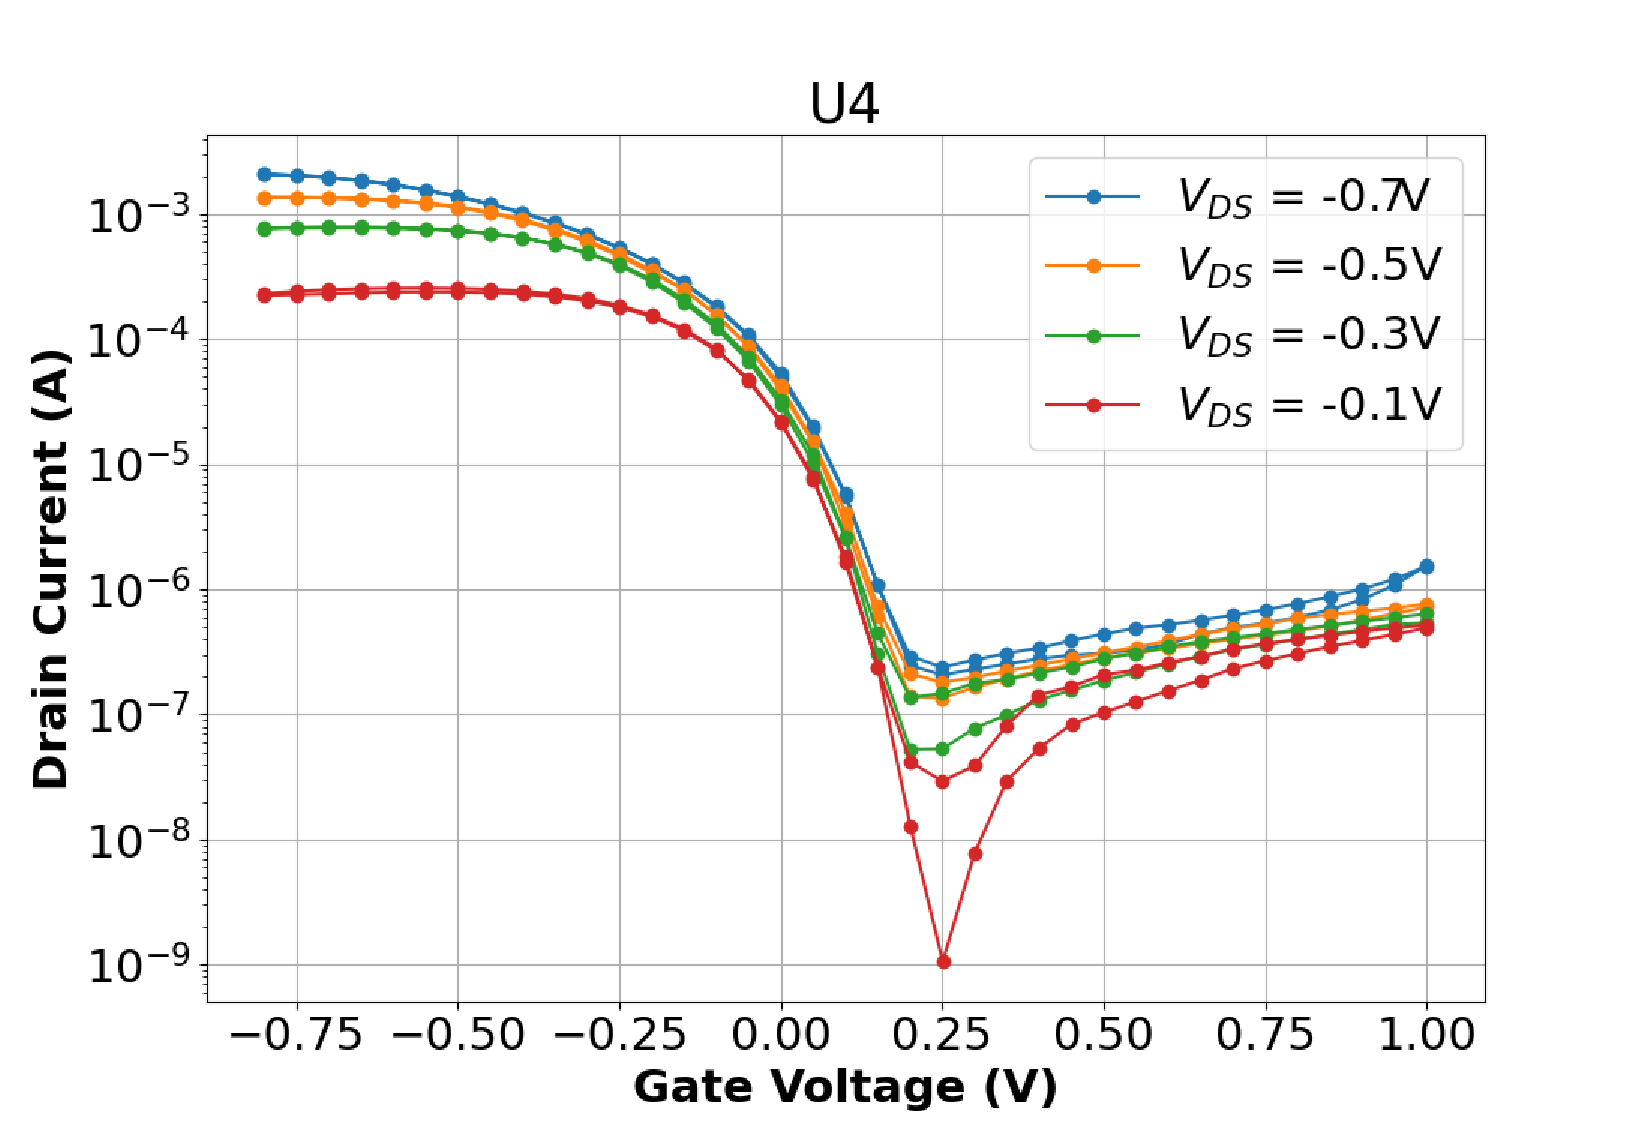
\includegraphics[height=5.2cm]{Images/pdf/transfer_undoped.pdf} }}
    \subfloat[Undoped device]{{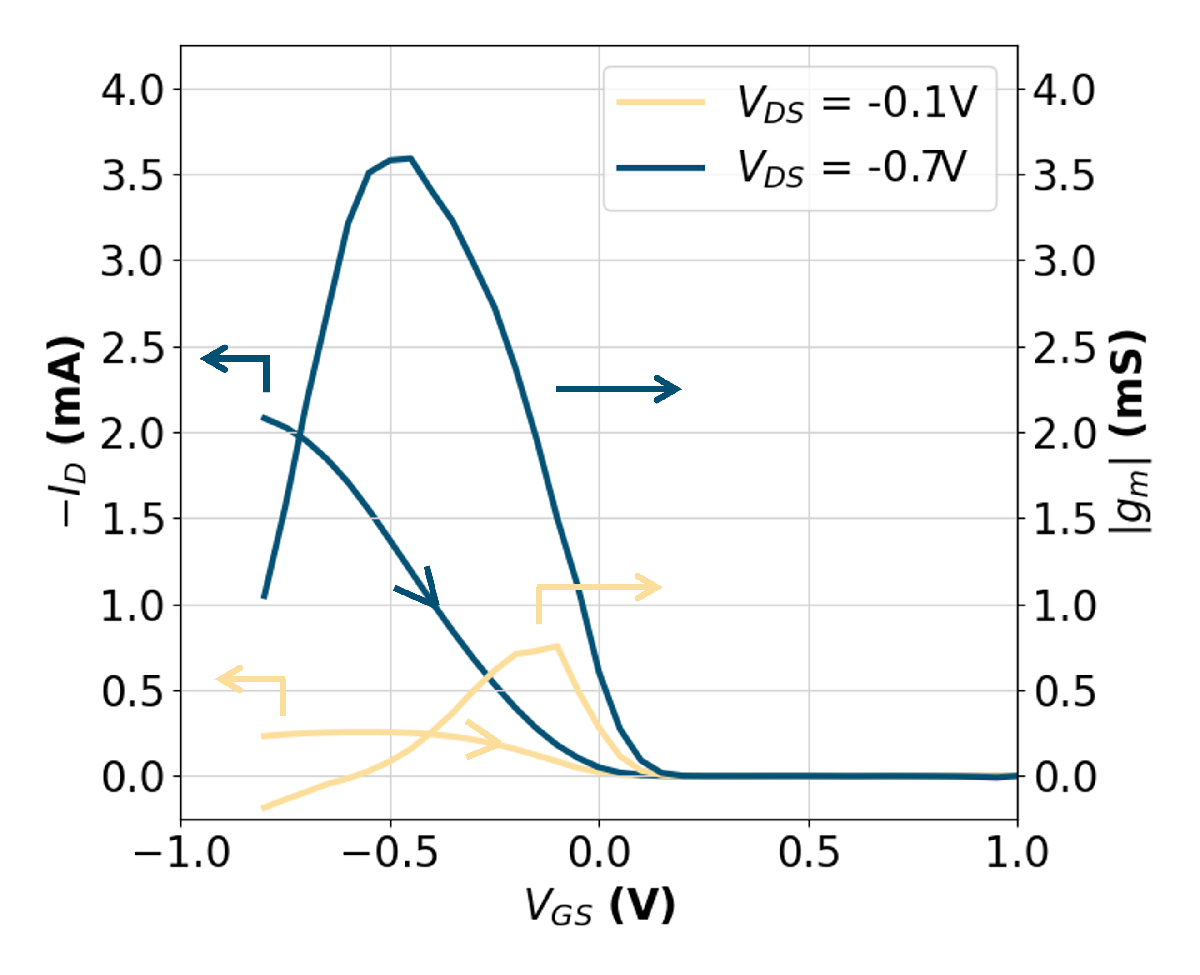
\includegraphics[height=5.0cm]{Images/pdf/id+gm_undoped_final.pdf} }}
    \qquad
    \subfloat[5 mg/mL dopant device]{{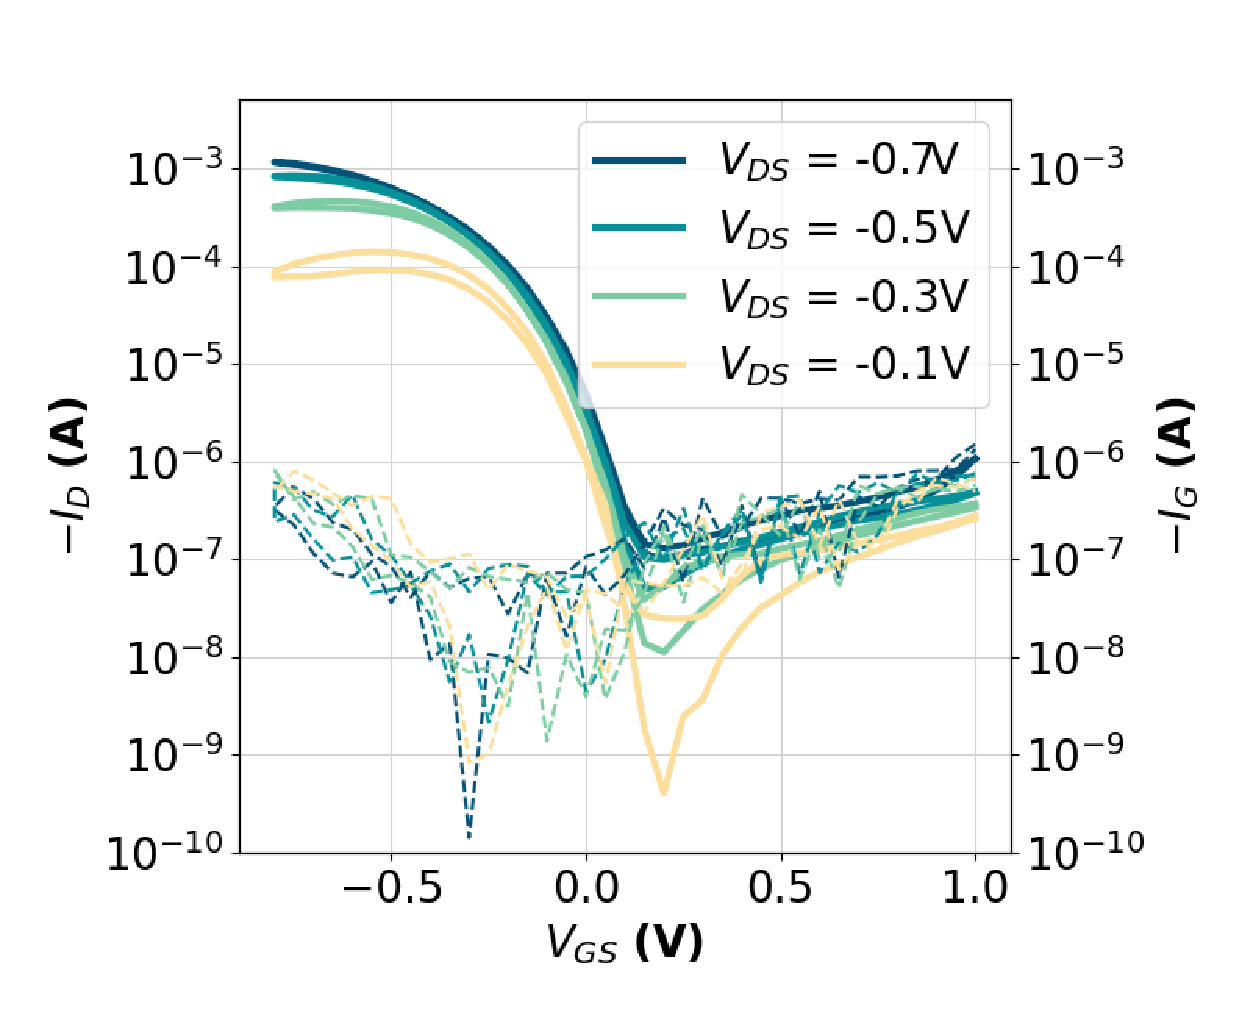
\includegraphics[height=5.2cm]{Images/pdf/transfer_doped5.pdf} }}
    \subfloat[5 mg/mL dopant device]{{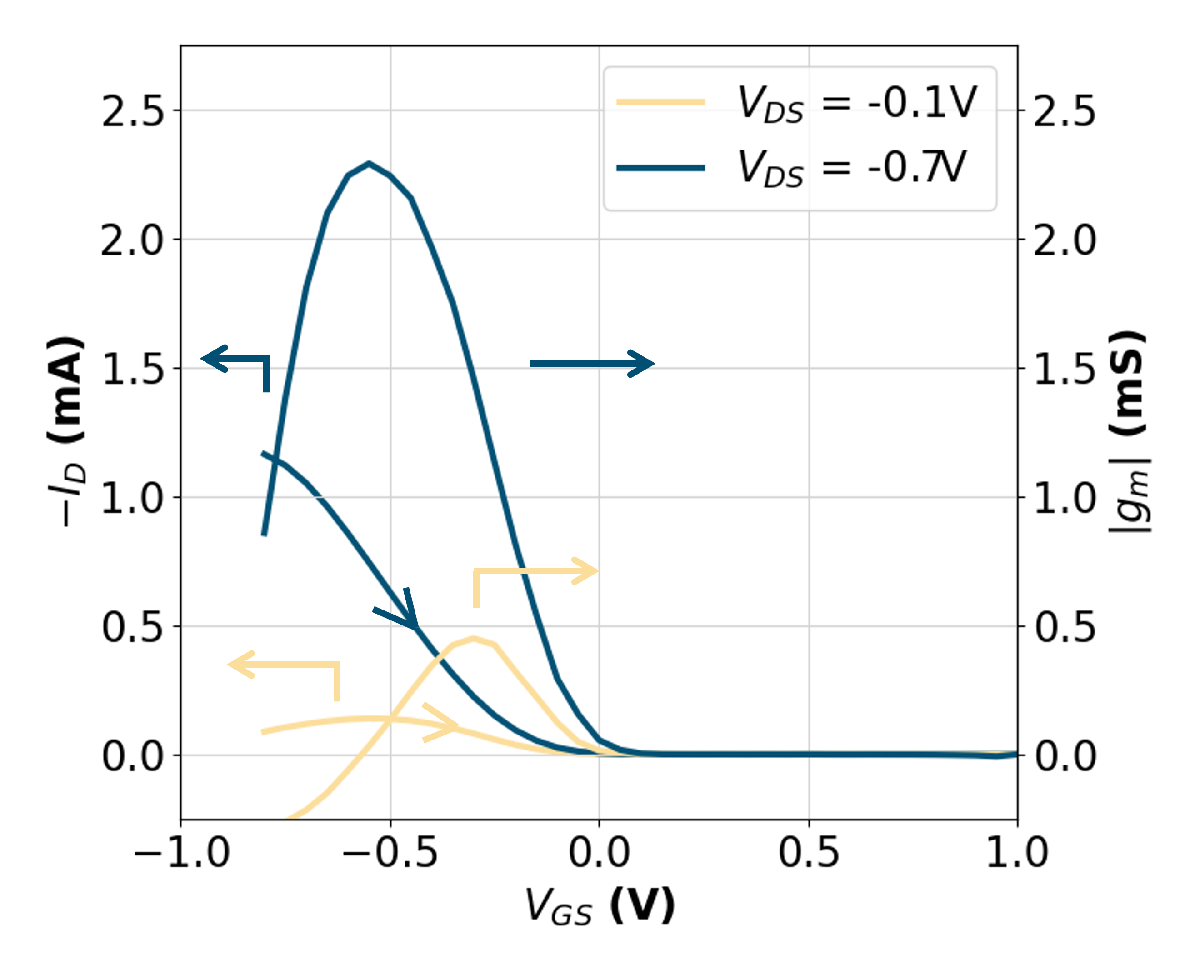
\includegraphics[height=5.0cm]{Images/pdf/id+gm_doped5_final.pdf} }}
    \qquad
    \subfloat[10 mg/mL dopant device]{{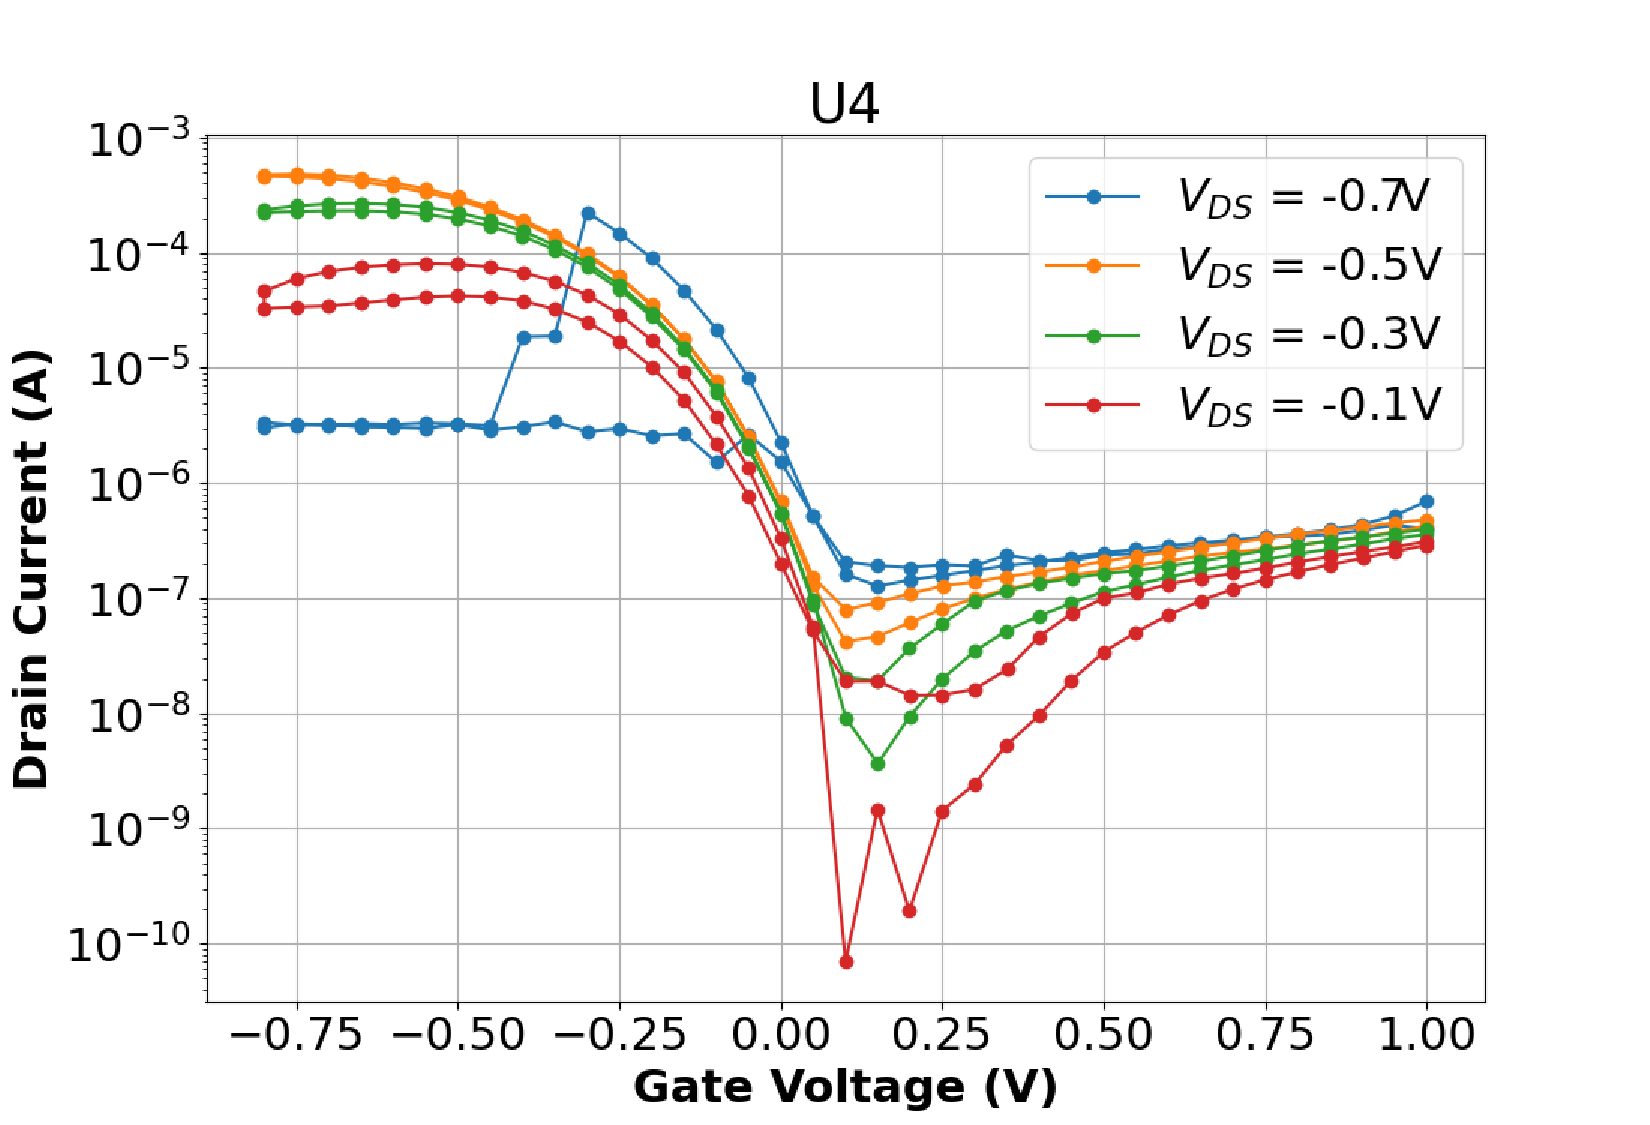
\includegraphics[height=5.2cm]{Images/pdf/transfer_doped10.pdf} }}
    \subfloat[10 mg/mL dopant device]{{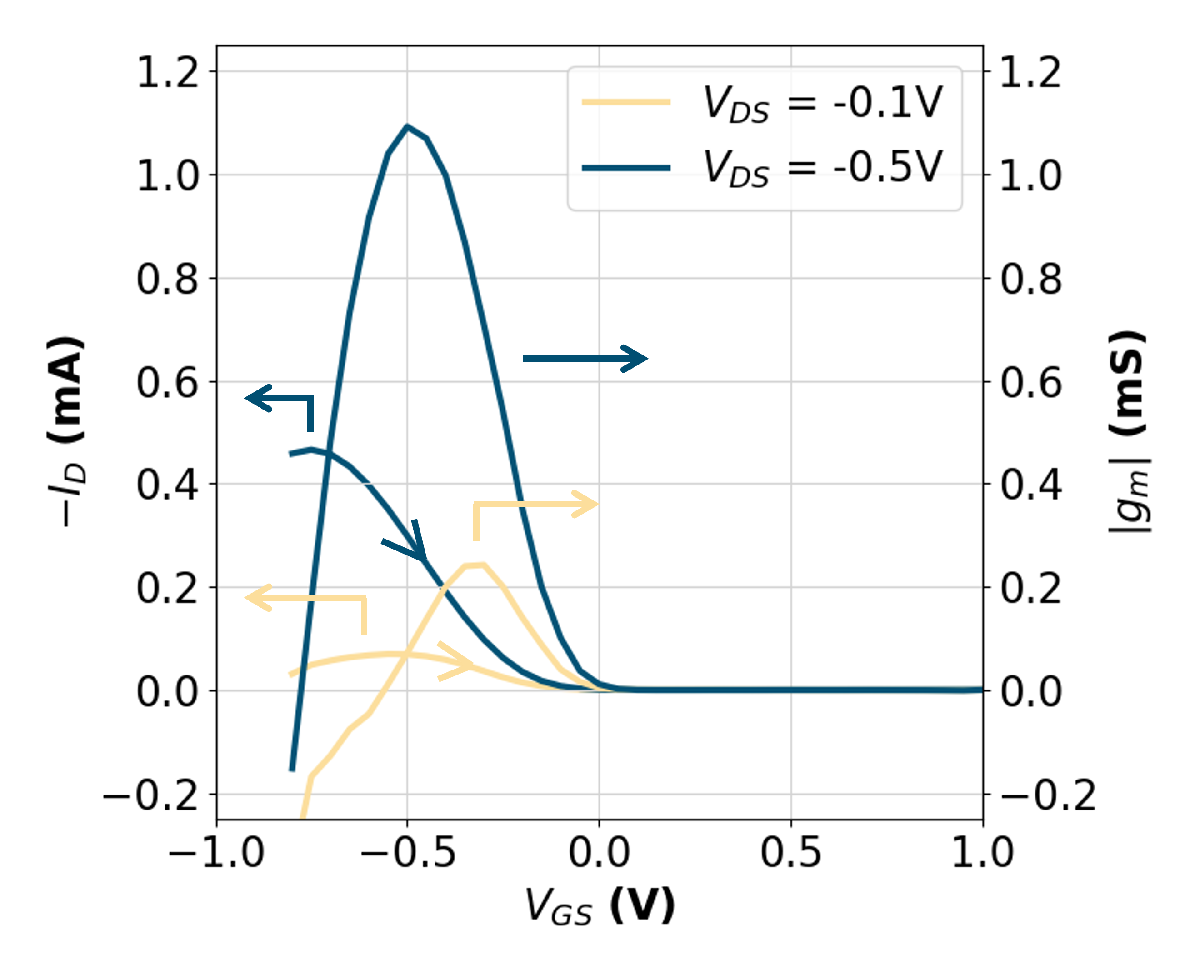
\includegraphics[height=5.0cm]{Images/pdf/id+gm_doped10_final.pdf} }}
    \caption[Transfer characteristics and transconductance at different doping levels and V$_{DS}$]{A), C), E) Transfer characteristics of all measured V$_{DS}$ including the gate leakage current I$_{G}$ B), D), F) Transfer curves (off-switching) with corresponding transconductance. Each group of graphs for undoped, 5 mg/mL and 10 mg/mL doped p(g3T2-T) channel, respectively.}
    \label{fig:transx2}
\end{figure}

%U4 loop 2 as undoped pattern
%U2 loop 3 for doped 5
%U4 loop 3 for doped 10

Additionally, it is observed that I$_{DS,ON}$ decreases while increasing doping levels. This is reflected in the maximum transconductance values displayed in Table \ref{tab:trans}. Additionally to the oxidation of undoped p(g3T2-T) devices that also increased I$_{DS,OFF}$. When doping our polymer, we are increasing its conductivity by inducing new charges in its backbone, the introduction of new ionic species will negatively impact the mobility of the induced charges, which explains the decrease in I$_{DS,ON}$. 

\begin{table}[ht]
\centering
\caption{Maximum transconductance values extracted from Figure \ref{fig:transx2}}
\begin{tabular}{l|c|c|c}
|g$_{m,max}$| [mS] @ & Undoped & 5 mg/mL & 10 mg/mL \\\hline
V$_{DS}$ = -0.1 V & 0.75 & 0.45 & 0.24\\
V$_{DS}$ = -0.3 V & 2.01 & 1.31 & 0.74\\
V$_{DS}$ = -0.5 V & 2.90 & 1.97 & 1.09\\
V$_{DS}$ = -0.7 V & 3.59 & 2.23 & \\ \hline
\end{tabular}
\label{tab:trans}
\end{table}

More importantly and counterintuitive, Figure \ref{fig:shift1} and Figure \ref{fig:vth_vds} showed turn ON voltages and threshold voltages, respectively, \textbf{shifted towards negative values} as the dopant concentration increased in all V$_{DS}$ values. The introduction of ionic species (TCNQ$^{-}$) should have created depletion-mode devices, so a higher positive gate biased would have been needed to counteract anions and turn OFF the device, resulting to positive threshold voltage (which is the case of PEDOT:PSS, V$_{Th}$ of 0.6 - 0.7 V). However, a sort of \textit{compensation doping} happened upon coupling channel and gate with SSE precursor, and as explained in the Background chapter, p(g3T2-T) as a type VI OMIEC, unlike PEDOT:PSS, have ionic species as free carriers and not chemically bonded. Further analysis in the conductivity needs to be done to understand to impact of this coupling in our undoped and doped polymer.
%% EG3 ensure no cation trapping in the crystalline phase of OMIECs

\begin{figure}[!ht]
    \centering
    \subfloat[V$_{DS}$ = -0.1 V]{{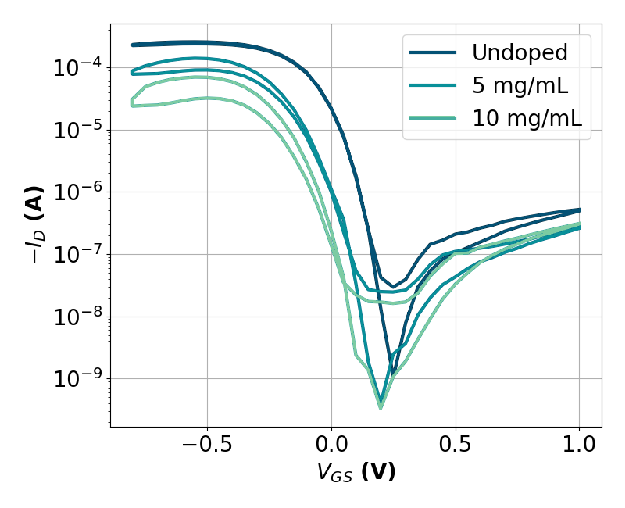
\includegraphics[height=5.5cm]{Images/pdf/Shift_Vds1.pdf} }}
    \subfloat[V$_{DS}$ = -0.3 V]{{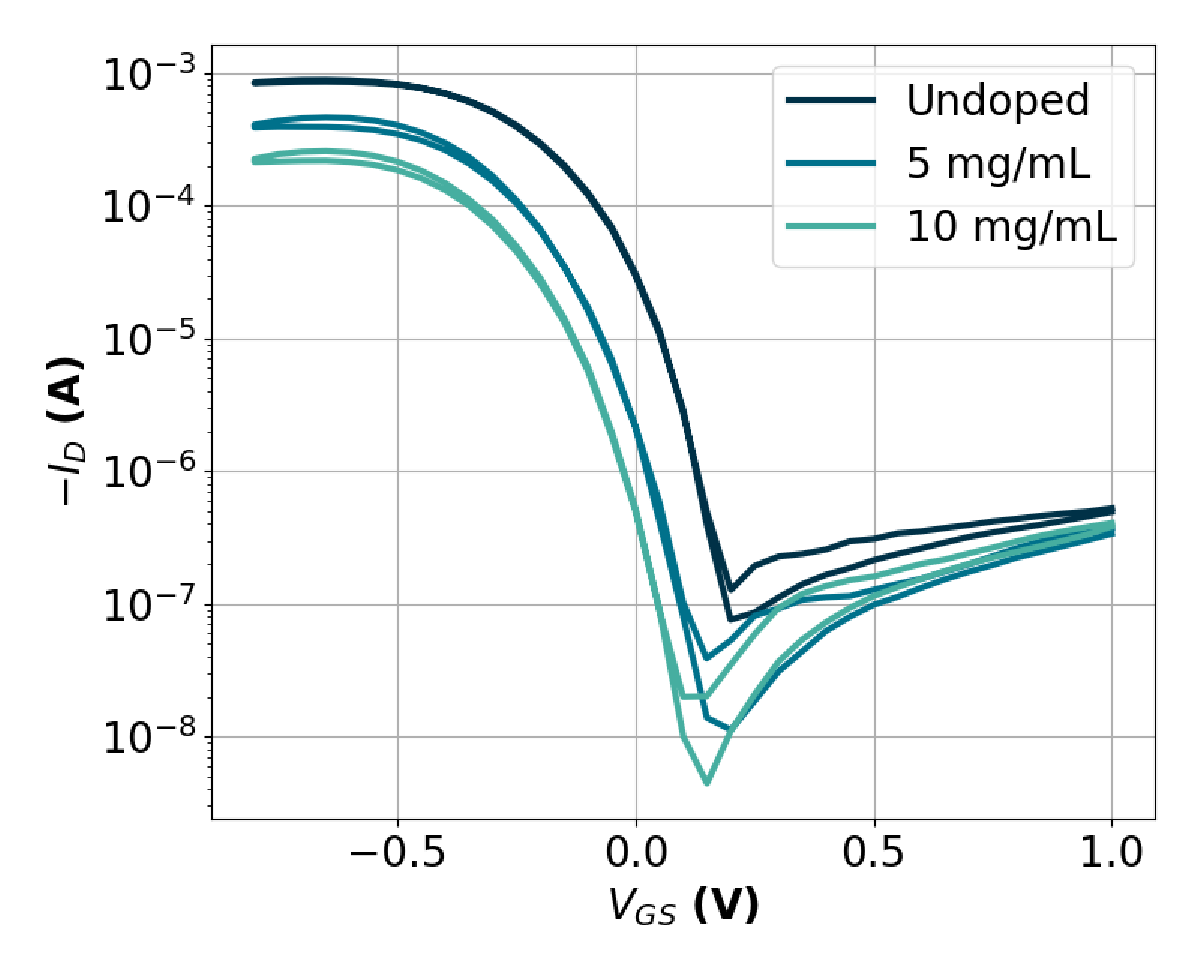
\includegraphics[height=5.5cm]{Images/pdf/Shift_Vds3.pdf} }}
    \qquad
    \subfloat[V$_{DS}$ = -0.5 V]{{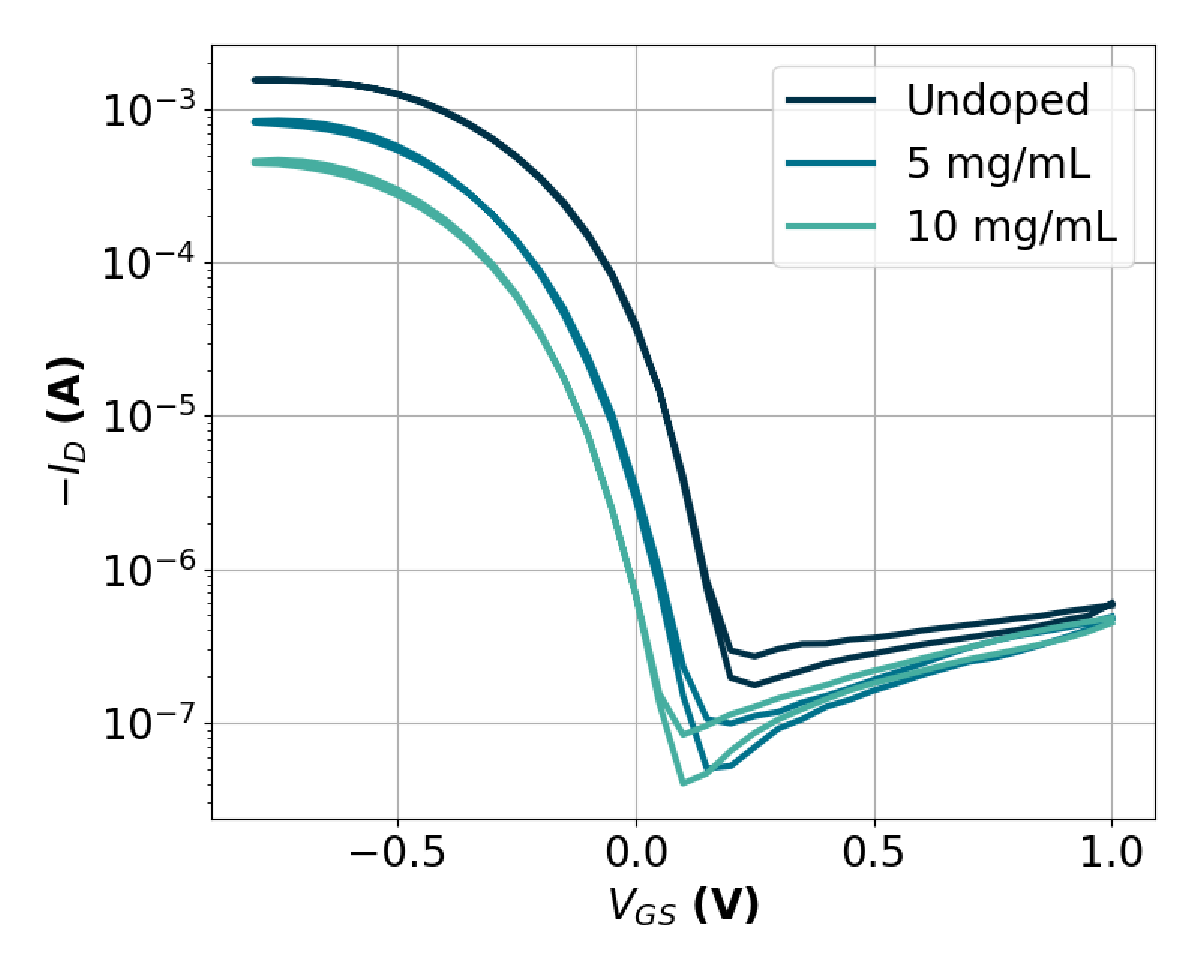
\includegraphics[height=5.5cm]{Images/pdf/Shift_Vds5.pdf} }}
    \subfloat[V$_{DS}$ = -0.7 V]{{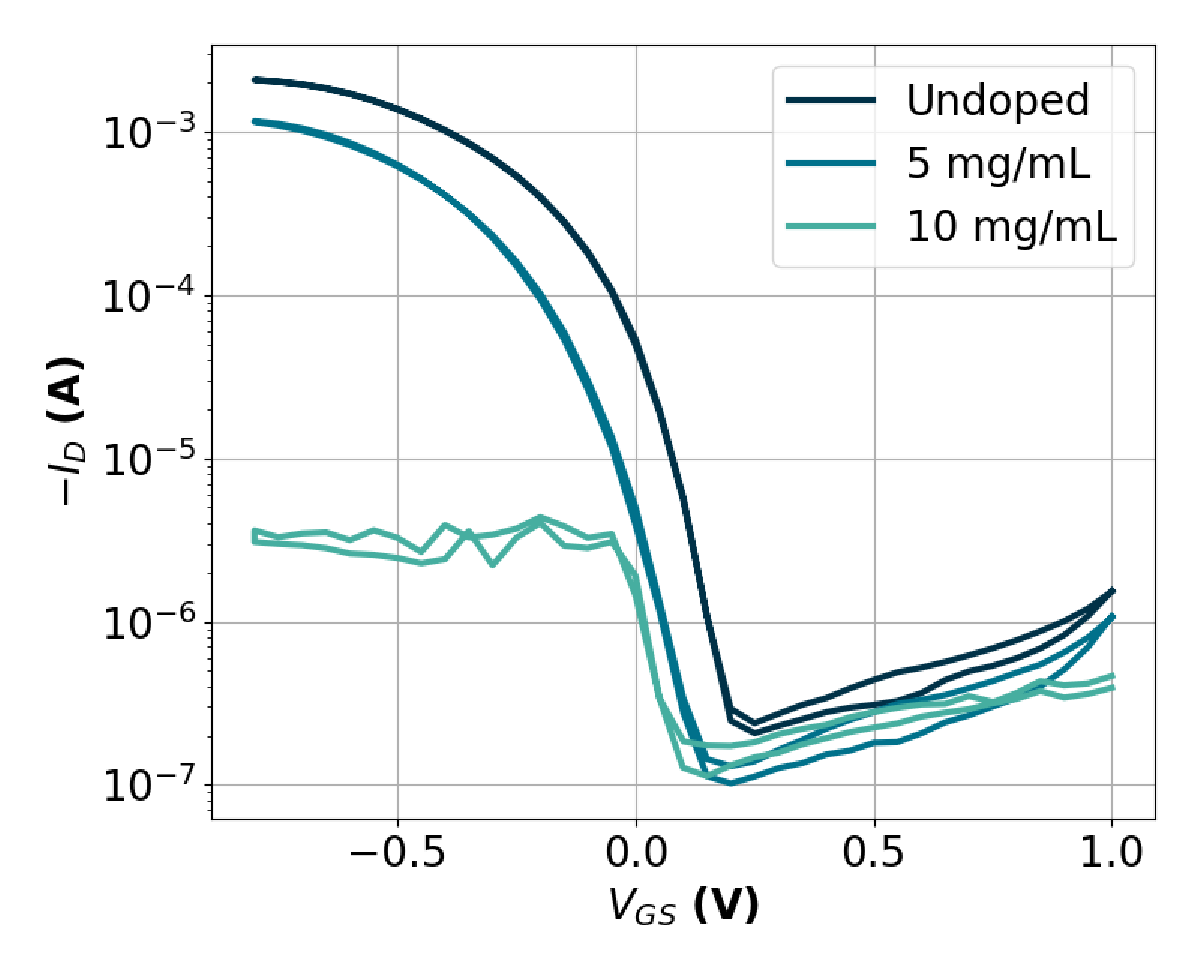
\includegraphics[height=5.5cm]{Images/pdf/Shift_Vds7.pdf} }}
    \caption[Transfer characteristics comparing different doping levels]{Transfer characteristics comparing undoped, 5 mg/mL and 10 mg/mL dopants devices, each graph represent a different V$_{DS }$}
    \label{fig:shift1}
\end{figure}

\begin{figure}[ht]
  \centering
  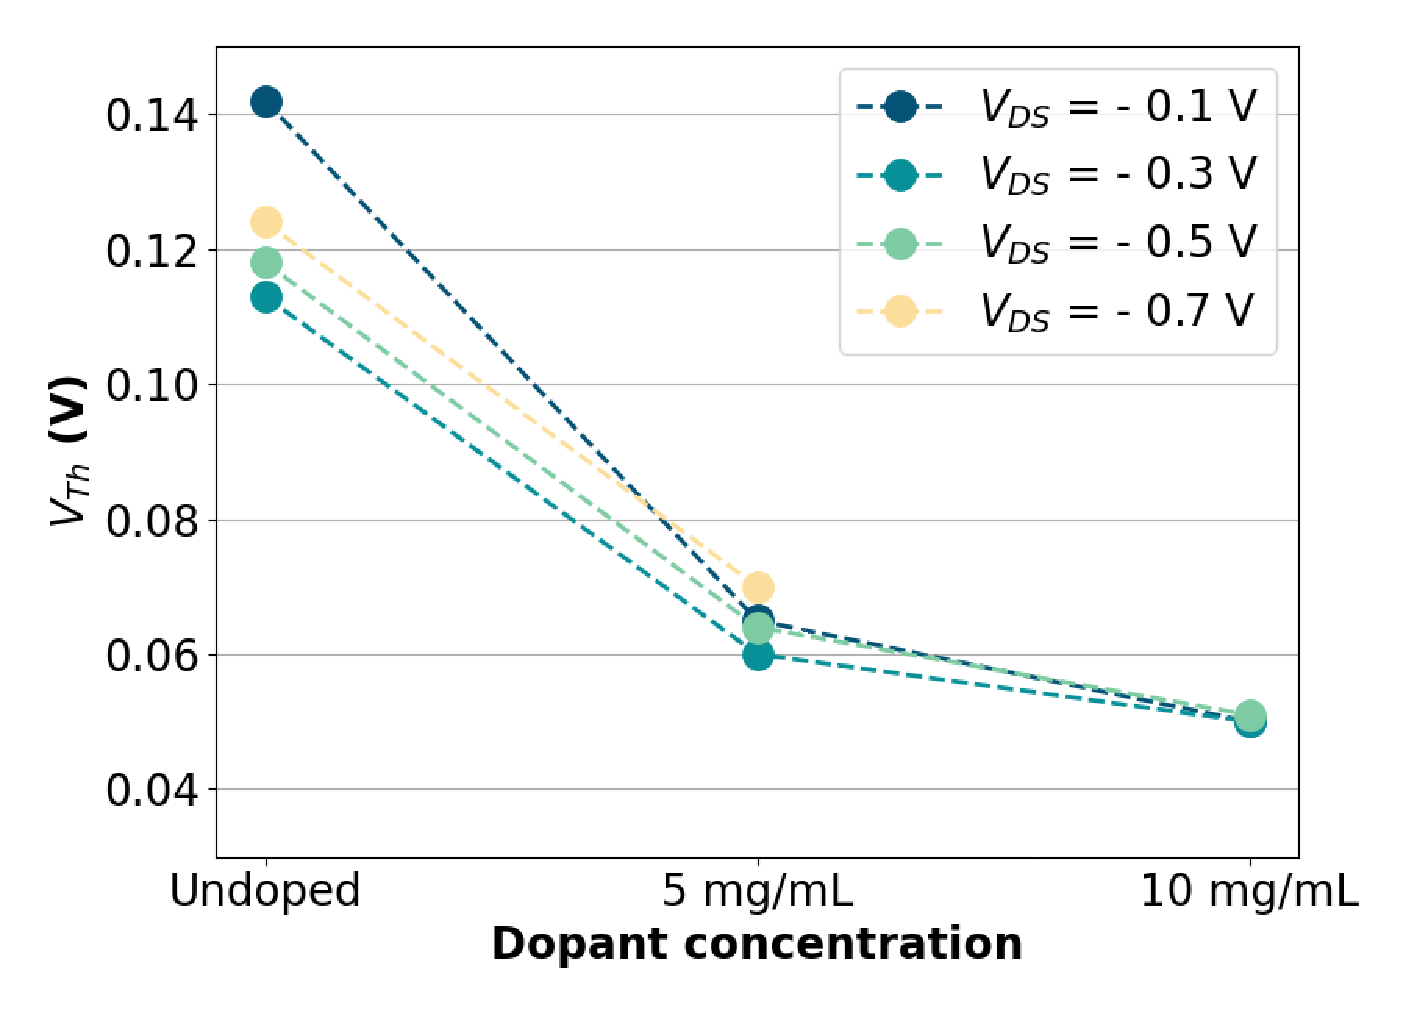
\includegraphics[width=10cm]{Images/pdf/vth_shift_vds.pdf}
  \caption[Threshold shift at different doping levels and V$_{DS}$]{Threshold shift at different doping levels and V$_{DS}$, corresponding from Figure \ref{fig:transx2}}
  \label{fig:vth_vds}
\end{figure}

Additionally, threshold values had lower variability among different values of V$_{DS}$ with higher introduction of dopants (Figure \ref{fig:vth_vds}). This variability could be caused by ORR which should be different at different biased conditions. By bringing the polymer towards its HOMO level by doping, we assured a better stability in air, then although we are impacting mobility and repeatibility among loops, the values at different drain biased are maintain.

Moreover, something that it is not shown in this report but it was perceived during analysis, there is higher repeatability of transfer characteristics with undoped OECT devices. This could be explained by considering our environmental conditions as a infinite reservoir of molecular oxygen, until this unwanted doping and ORR reaches saturation, making it stable. In the case of F$_{4}$TCNQ, stability is still unclear and further investigation will be done in the next sections.

\subsection{Stability on Air of p(g3T2-T)}

Channel conductivity was measured before and after the patterning process. Immediately after spin-coating unpatterned p(g3T2-T) exhibited a conductivity around 1 $\mu$S, after patterning the conductivity increase to three orders of magnitude to the order of 1 mS, a clear sign of oxidation after the whole patterning process. Measurements of I$_{D}$ at -0.3 V of V$_{DS}$ and no gate biased in glovebox exhibited a small decrease of 4\% within two hours, and small increase of 15\% within two hours in air exposure, pretty stable after patterning.

Interestingly, upon contact with SSE precursor, conductivity drops significantly, at least six orders of magnitude, as shown in Figure \ref{fig:revox1}A. Another device from another sample was tested showing the same result. 

%\begin{table}[ht]
%\centering
%\caption{Conductivity measurements of undoped p(g3T2-T)}
%\begin{tabular}{l|c}
%Condition  & Conductivity (S) \\\hline
%Unpatterned & 1.3 $\times$ 10^{-6} \\
%Patterned & 1.0 $\times$ 10^{-3} \\
%\end{tabular}
%\label{tab:cond}
%\end{table}

Transfer curves were measured from the latter device under environmental conditions with a Ag/AgCl pellet, a clear shift to more negative values of turn ON values are noticed, as reported in Figure \ref{fig:revox1}B.


\begin{figure}[!ht]
    \centering
    \subfloat[N$_{2}$ environment]{{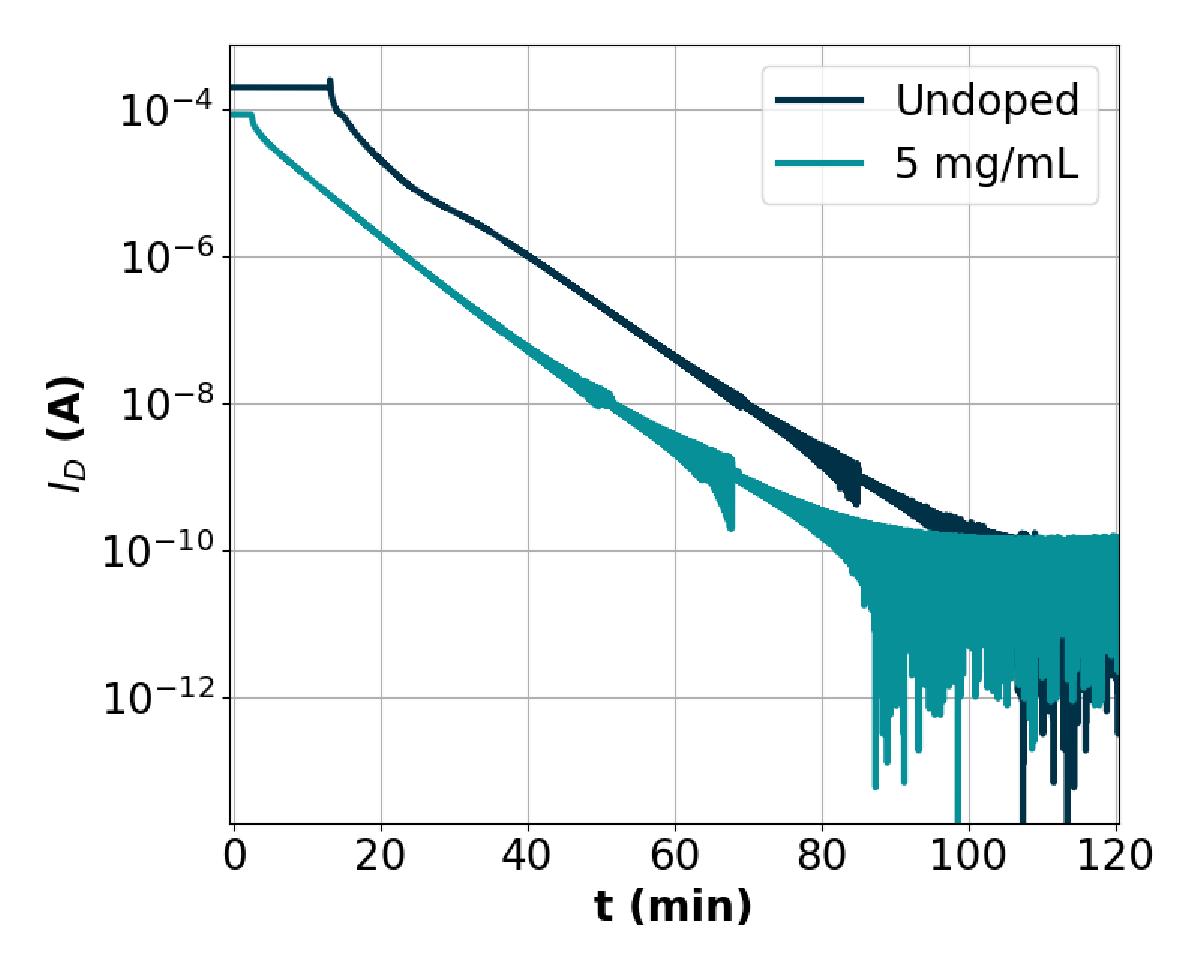
\includegraphics[height=5.5cm]{Images/pdf/revox_gb_only.pdf} }}
    \subfloat[Ambient environment]{{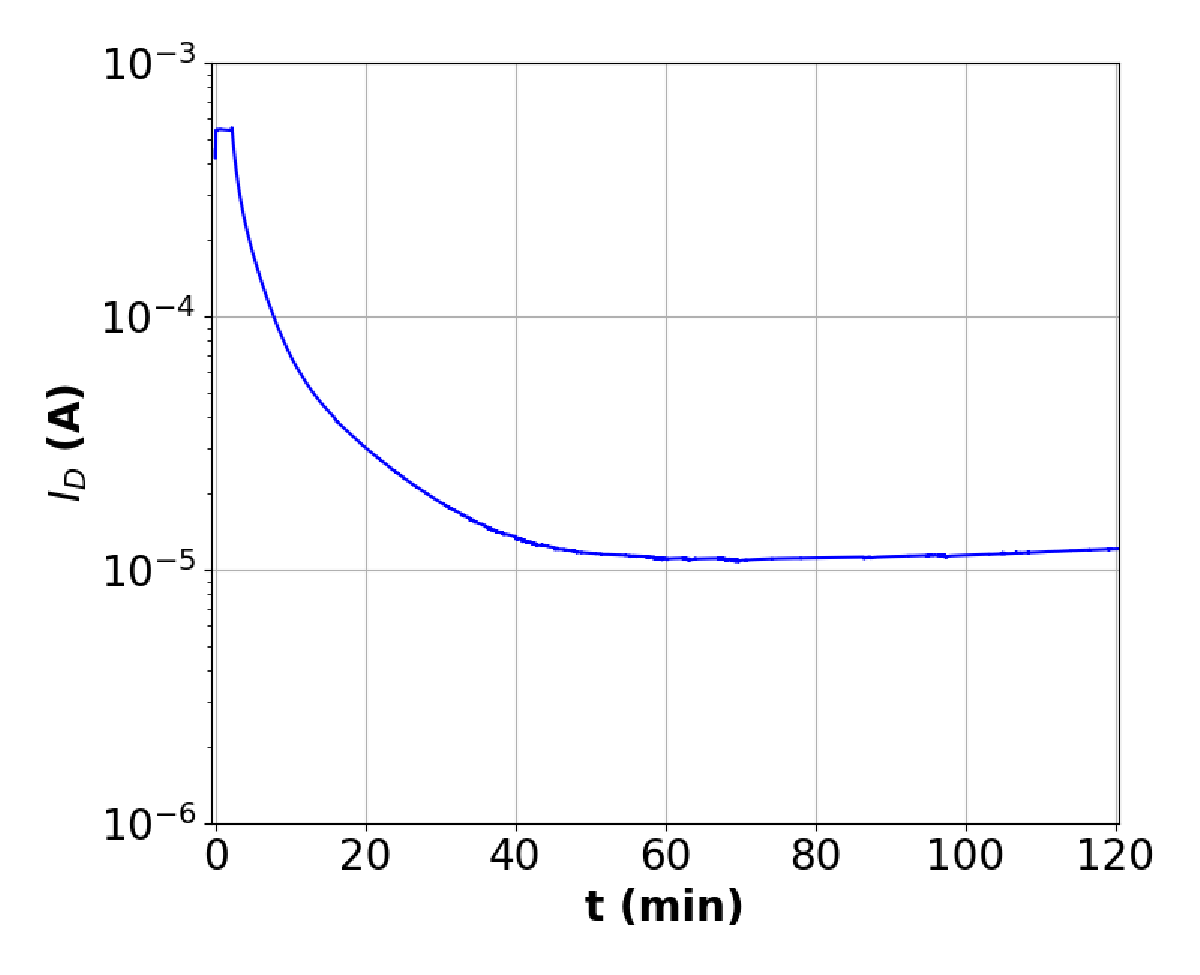
\includegraphics[height=5.5cm]{Images/pdf/revox_air.pdf} }}
    \subfloat[Ambient + N$_{2}$ environment]{{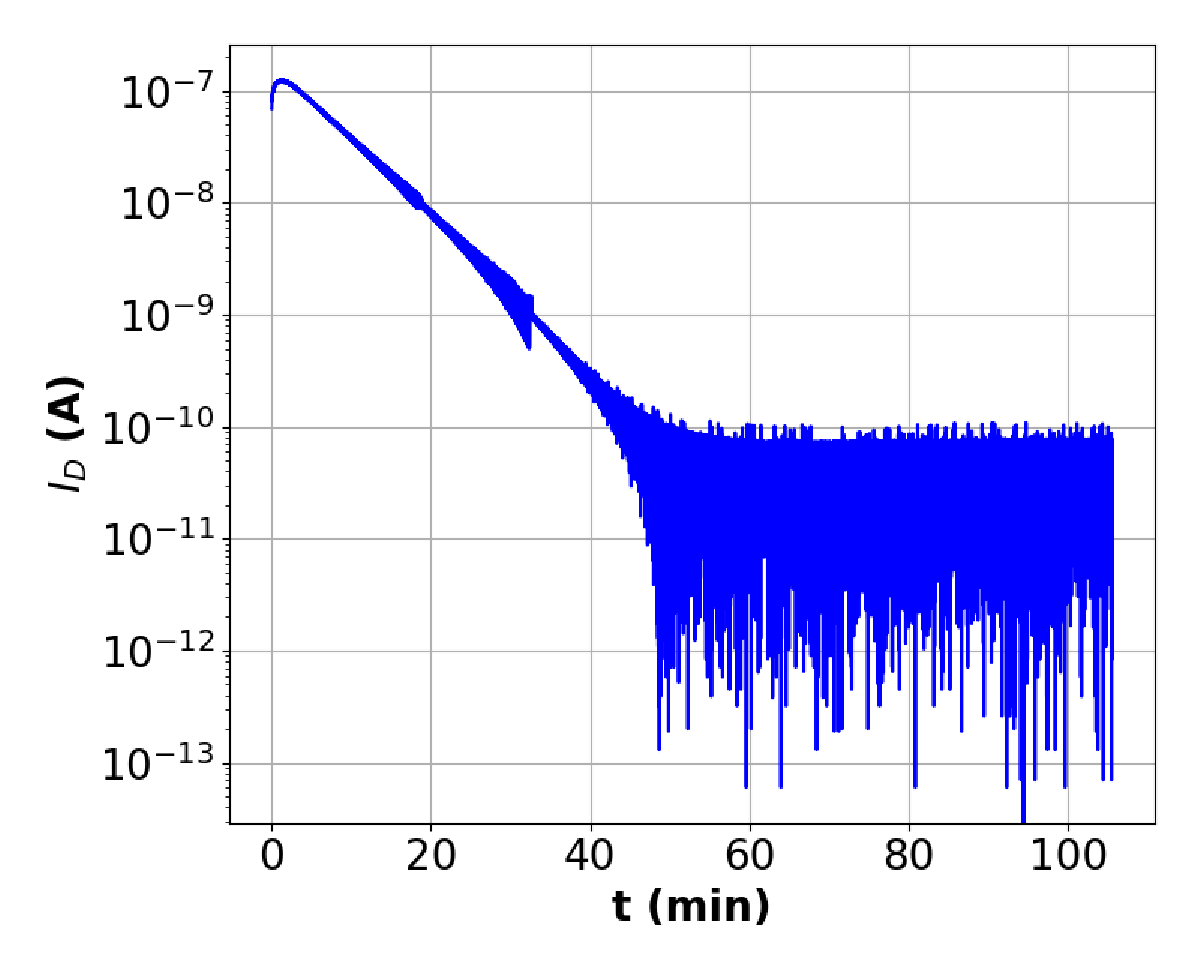
\includegraphics[height=5.5cm]{Images/pdf/revox_gb_afterair.pdf} }}
    \caption[Transfer characteristics comparing different doping levels]{Transfer characteristics comparing undoped, 5 mg/mL and 10 mg/mL dopants devices, each graph represent a different V$_{DS }$}
    \label{fig:revox1}
\end{figure}


\subsection{Reverse Oxidation of Undoped-p(g3T2-T)}


\begin{figure}[!ht]
    \centering
    \subfloat[N$_{2}$ environment]{{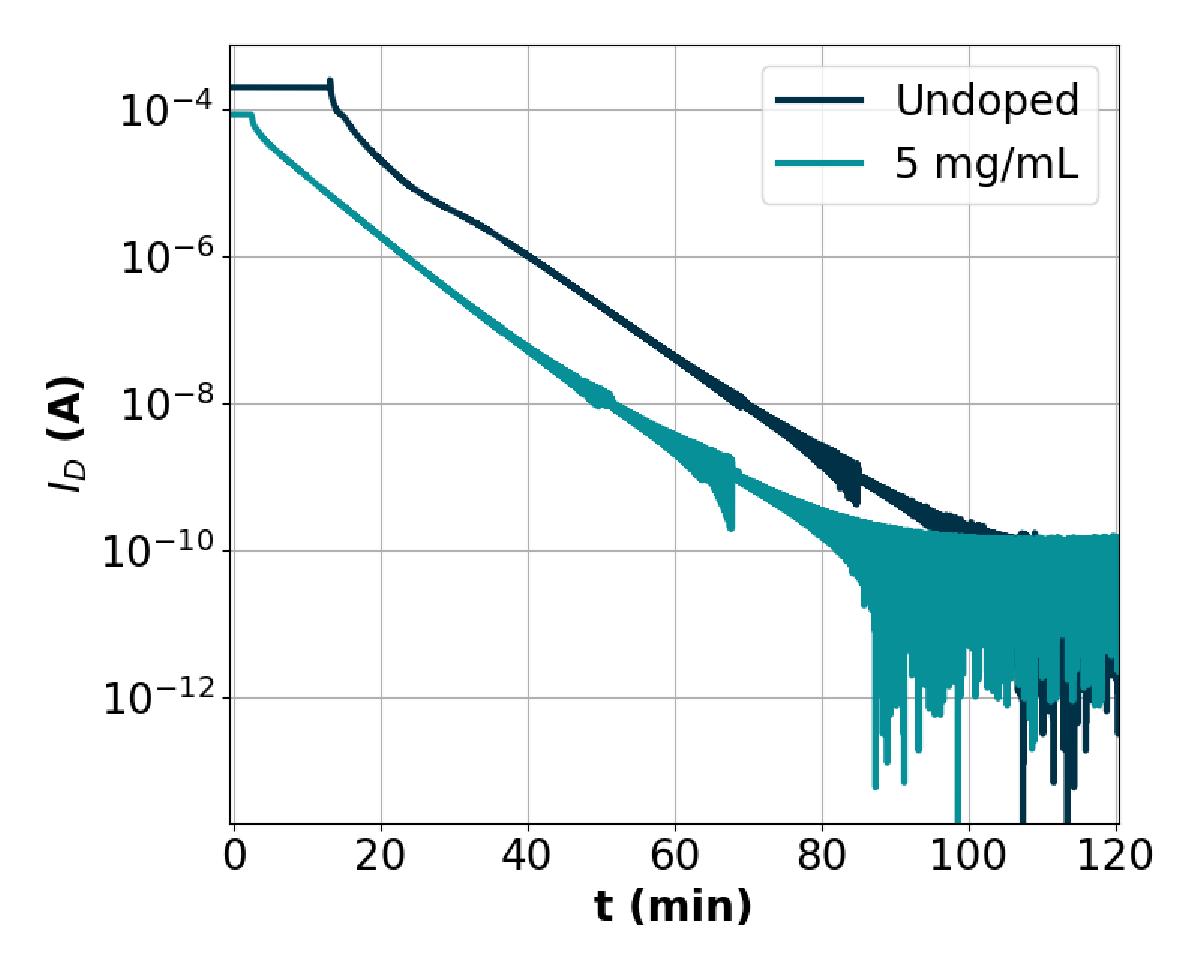
\includegraphics[height=5.5cm]{Images/pdf/revox_gb_only.pdf} }}
    \subfloat[Transfer in ambient]{{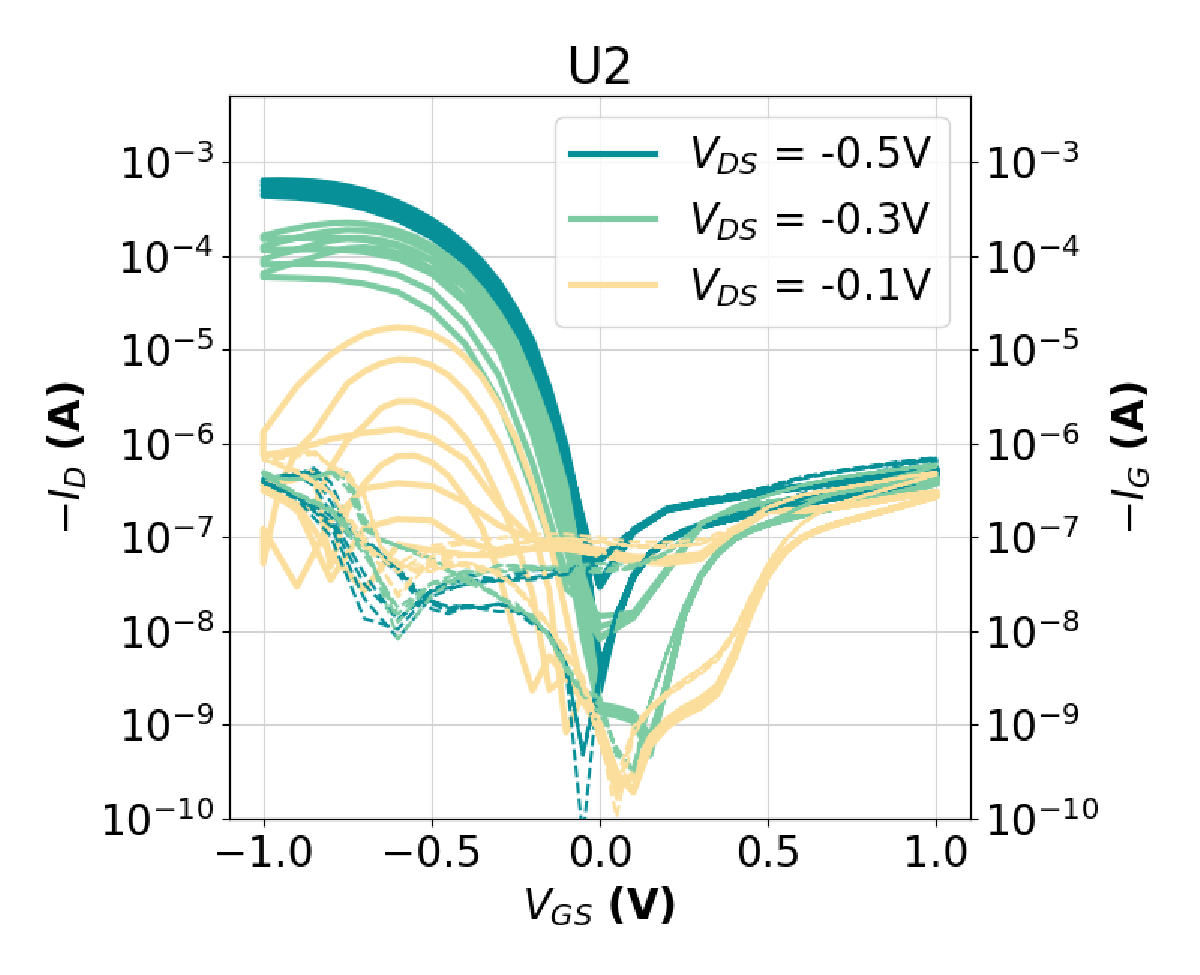
\includegraphics[height=5.5cm]{Images/pdf/revox_transfer_loops1.pdf} }}
    \caption[Reversing oxidation of undoped-p(g3T2-T)]{Transfer characteristics comparing undoped, 5 mg/mL and 10 mg/mL dopants devices, each graph represent a different V$_{DS }$}
    \label{fig:revox2}
\end{figure}

\subsubsection{By Electrochemical Dedoping}

\subsubsection{By Heating}


\subsection{Solid-OECTs using Undoped p(g3T2-T)}


%The Ag/AgCl gate electrode’s work function is reasonably constant, the work function of an OMIEC gate electrode however may vary depending on its processing history and redox reactions with other species present in the electrolyte (e.g. molecular oxygen).28 Applying VGS only determines the potential difference between the gate and channel but does not control the potentials of either electrode (hence the position of the Fermi level) with respect to a reference. This leads to many challenges in operating an OECT with OMIEC gate electrodes.


\subsubsection{Dropcasted Solid-State Electrolyte}

\subsubsection{OECT with Dropcast Solid-State Electrolyte}

\subsubsection{OECT with Photopatternable Solid-State Electrolyte}

\subsubsection{OECT with Inkjet-Printed Solid-State Electrolyte}


\subsection{Solid-OECTs using Doped-p(g3T2-T)}



%Achieving effective charge transfer between the analyte and OMIEC requires appropriate alignment of the electrochemical potential of electrons on the OMIEC electrode and the redox specie. Failure to do so may result in the subsequent transfer of charges to other redox-active sinks in the environment, leading to undesirable side reactions and products that may interfere with the OMIEC’s operation. Electrons flow from a region of higher to lower electrochemical potential. Hence, achieving electron transfer from redox-active species to the OMIEC requires the latter to have a deep LUMO (high electron affinity) \cite{tanMixedIonicElectronic2022} %paper

%\section{Conclusion}
%\lipsum[86-88]

%%% Local Variables: 
%%% mode: latex
%%% TeX-master: "thesis"
%%% End: 
